% Options for packages loaded elsewhere
\PassOptionsToPackage{unicode}{hyperref}
\PassOptionsToPackage{hyphens}{url}
%
\documentclass[
]{article}
\usepackage{lmodern}
\usepackage{amssymb,amsmath}
\usepackage{ifxetex,ifluatex}
\ifnum 0\ifxetex 1\fi\ifluatex 1\fi=0 % if pdftex
  \usepackage[T1]{fontenc}
  \usepackage[utf8]{inputenc}
  \usepackage{textcomp} % provide euro and other symbols
\else % if luatex or xetex
  \usepackage{unicode-math}
  \defaultfontfeatures{Scale=MatchLowercase}
  \defaultfontfeatures[\rmfamily]{Ligatures=TeX,Scale=1}
\fi
% Use upquote if available, for straight quotes in verbatim environments
\IfFileExists{upquote.sty}{\usepackage{upquote}}{}
\IfFileExists{microtype.sty}{% use microtype if available
  \usepackage[]{microtype}
  \UseMicrotypeSet[protrusion]{basicmath} % disable protrusion for tt fonts
}{}
\makeatletter
\@ifundefined{KOMAClassName}{% if non-KOMA class
  \IfFileExists{parskip.sty}{%
    \usepackage{parskip}
  }{% else
    \setlength{\parindent}{0pt}
    \setlength{\parskip}{6pt plus 2pt minus 1pt}}
}{% if KOMA class
  \KOMAoptions{parskip=half}}
\makeatother
\usepackage{xcolor}
\IfFileExists{xurl.sty}{\usepackage{xurl}}{} % add URL line breaks if available
\IfFileExists{bookmark.sty}{\usepackage{bookmark}}{\usepackage{hyperref}}
\hypersetup{
  pdftitle={Combined Report: LN SED},
  pdfauthor={Kaveh G. Siah},
  hidelinks,
  pdfcreator={LaTeX via pandoc}}
\urlstyle{same} % disable monospaced font for URLs
\usepackage[margin=2 cm]{geometry}
\usepackage{graphicx}
\makeatletter
\def\maxwidth{\ifdim\Gin@nat@width>\linewidth\linewidth\else\Gin@nat@width\fi}
\def\maxheight{\ifdim\Gin@nat@height>\textheight\textheight\else\Gin@nat@height\fi}
\makeatother
% Scale images if necessary, so that they will not overflow the page
% margins by default, and it is still possible to overwrite the defaults
% using explicit options in \includegraphics[width, height, ...]{}
\setkeys{Gin}{width=\maxwidth,height=\maxheight,keepaspectratio}
% Set default figure placement to htbp
\makeatletter
\def\fps@figure{htbp}
\makeatother
\setlength{\emergencystretch}{3em} % prevent overfull lines
\providecommand{\tightlist}{%
  \setlength{\itemsep}{0pt}\setlength{\parskip}{0pt}}
\setcounter{secnumdepth}{-\maxdimen} % remove section numbering
\usepackage{subfig}
\usepackage{booktabs}
\usepackage{longtable}
\usepackage{array}
\usepackage{multirow}
\usepackage{wrapfig}
\usepackage{float}
\usepackage{colortbl}
\usepackage{pdflscape}
\usepackage{tabu}
\usepackage{threeparttable}
\usepackage{threeparttablex}
\usepackage[normalem]{ulem}
\usepackage{makecell}
\usepackage{xcolor}
\ifluatex
  \usepackage{selnolig}  % disable illegal ligatures
\fi

\title{Combined Report: LN SED}
\author{Kaveh G. Siah}
\date{11/11/2020}

\begin{document}
\maketitle

\hypertarget{chapter-1}{%
\section{Chapter 1}\label{chapter-1}}

\newpage 
\tableofcontents
\listoffigures
\listoftables
\newpage

\hypertarget{soil-solution-results}{%
\subsubsection{Soil Solution Results}\label{soil-solution-results}}

\begin{table}[!h]

\caption{\label{tab:unnamed-chunk-6}Average Soil Solution Concentrations of Reliable Months (2005-2006)}
\centering
\resizebox{\linewidth}{!}{
\begin{tabular}[t]{lllllllllllllllll}
\toprule
\multicolumn{1}{c}{ } & \multicolumn{16}{c}{\$\textbackslash{}\textbackslash{}mu\$mol/L} \\
\cmidrule(l{3pt}r{3pt}){2-17}
Soil Layer & Ca & Mg & K & Na & NO3 & NH4 & SO4 & Cl & PO4 & DOC & Al & Si & H+ & pH & R & HR\\
\midrule
\cellcolor{gray!6}{Layer 1} & \cellcolor{gray!6}{13.8} & \cellcolor{gray!6}{18.3} & \cellcolor{gray!6}{17.3} & \cellcolor{gray!6}{45.8} & \cellcolor{gray!6}{2.080} & \cellcolor{gray!6}{1.881} & \cellcolor{gray!6}{24.3} & \cellcolor{gray!6}{55.2} & \cellcolor{gray!6}{1.004} & \cellcolor{gray!6}{393} & \cellcolor{gray!6}{0.01503} & \cellcolor{gray!6}{12.3} & \cellcolor{gray!6}{17.29} & \cellcolor{gray!6}{4.76} & \cellcolor{gray!6}{40.8} & \cellcolor{gray!6}{15.3}\\
Layer 2 & 16.4 & 22.5 & 19.1 & 54.8 & 1.437 & 1.014 & 25.3 & 63.0 & 0.886 & 630 & 0.02906 & 29.5 & 24.51 & 4.61 & 62.3 & 27.8\\
\cellcolor{gray!6}{Layer 3} & \cellcolor{gray!6}{22.9} & \cellcolor{gray!6}{27.0} & \cellcolor{gray!6}{22.2} & \cellcolor{gray!6}{49.5} & \cellcolor{gray!6}{1.036} & \cellcolor{gray!6}{0.708} & \cellcolor{gray!6}{25.3} & \cellcolor{gray!6}{69.1} & \cellcolor{gray!6}{0.716} & \cellcolor{gray!6}{691} & \cellcolor{gray!6}{0.01850} & \cellcolor{gray!6}{42.2} & \cellcolor{gray!6}{19.13} & \cellcolor{gray!6}{4.72} & \cellcolor{gray!6}{70.6} & \cellcolor{gray!6}{28.1}\\
Layer 4 & 9.2 & 16.0 & 14.6 & 47.5 & 0.618 & 0.754 & 12.9 & 65.6 & 0.395 & 421 & 0.02402 & 51.2 & 20.82 & 4.68 & 41.9 & 18.2\\
\cellcolor{gray!6}{Layer 5} & \cellcolor{gray!6}{12.8} & \cellcolor{gray!6}{21.1} & \cellcolor{gray!6}{14.9} & \cellcolor{gray!6}{50.5} & \cellcolor{gray!6}{0.545} & \cellcolor{gray!6}{1.331} & \cellcolor{gray!6}{12.7} & \cellcolor{gray!6}{71.1} & \cellcolor{gray!6}{0.184} & \cellcolor{gray!6}{421} & \cellcolor{gray!6}{0.00621} & \cellcolor{gray!6}{53.2} & \cellcolor{gray!6}{9.05} & \cellcolor{gray!6}{5.04} & \cellcolor{gray!6}{46.4} & \cellcolor{gray!6}{13.7}\\
\addlinespace
Layer 6 & 12.0 & 19.1 & 16.9 & 53.1 & 0.529 & 1.550 & 12.7 & 76.5 & 0.220 & 384 & 0.00762 & 56.9 & 10.59 & 4.98 & 41.8 & 13.0\\
\cellcolor{gray!6}{Layer 7} & \cellcolor{gray!6}{15.2} & \cellcolor{gray!6}{20.8} & \cellcolor{gray!6}{15.8} & \cellcolor{gray!6}{59.7} & \cellcolor{gray!6}{0.545} & \cellcolor{gray!6}{2.176} & \cellcolor{gray!6}{12.7} & \cellcolor{gray!6}{82.6} & \cellcolor{gray!6}{0.299} & \cellcolor{gray!6}{428} & \cellcolor{gray!6}{0.00473} & \cellcolor{gray!6}{61.3} & \cellcolor{gray!6}{7.32} & \cellcolor{gray!6}{5.14} & \cellcolor{gray!6}{48.3} & \cellcolor{gray!6}{12.8}\\
Layer 8 & 14.9 & 19.2 & 18.0 & 67.3 & 0.560 & 2.593 & 12.7 & 87.0 & 0.223 & 424 & 0.00363 & 63.7 & 5.91 & 5.23 & 49.0 & 11.7\\
\bottomrule
\end{tabular}}
\end{table}

\begin{figure}[H]
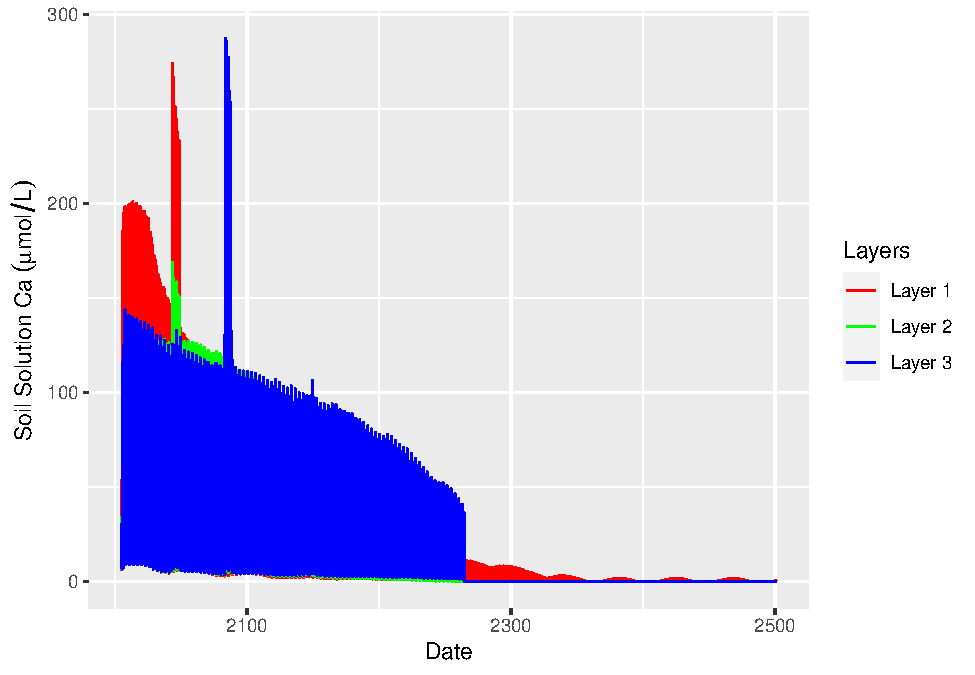
\includegraphics[width=0.5\linewidth]{Master_Report_files/figure-latex/figures-side-1} 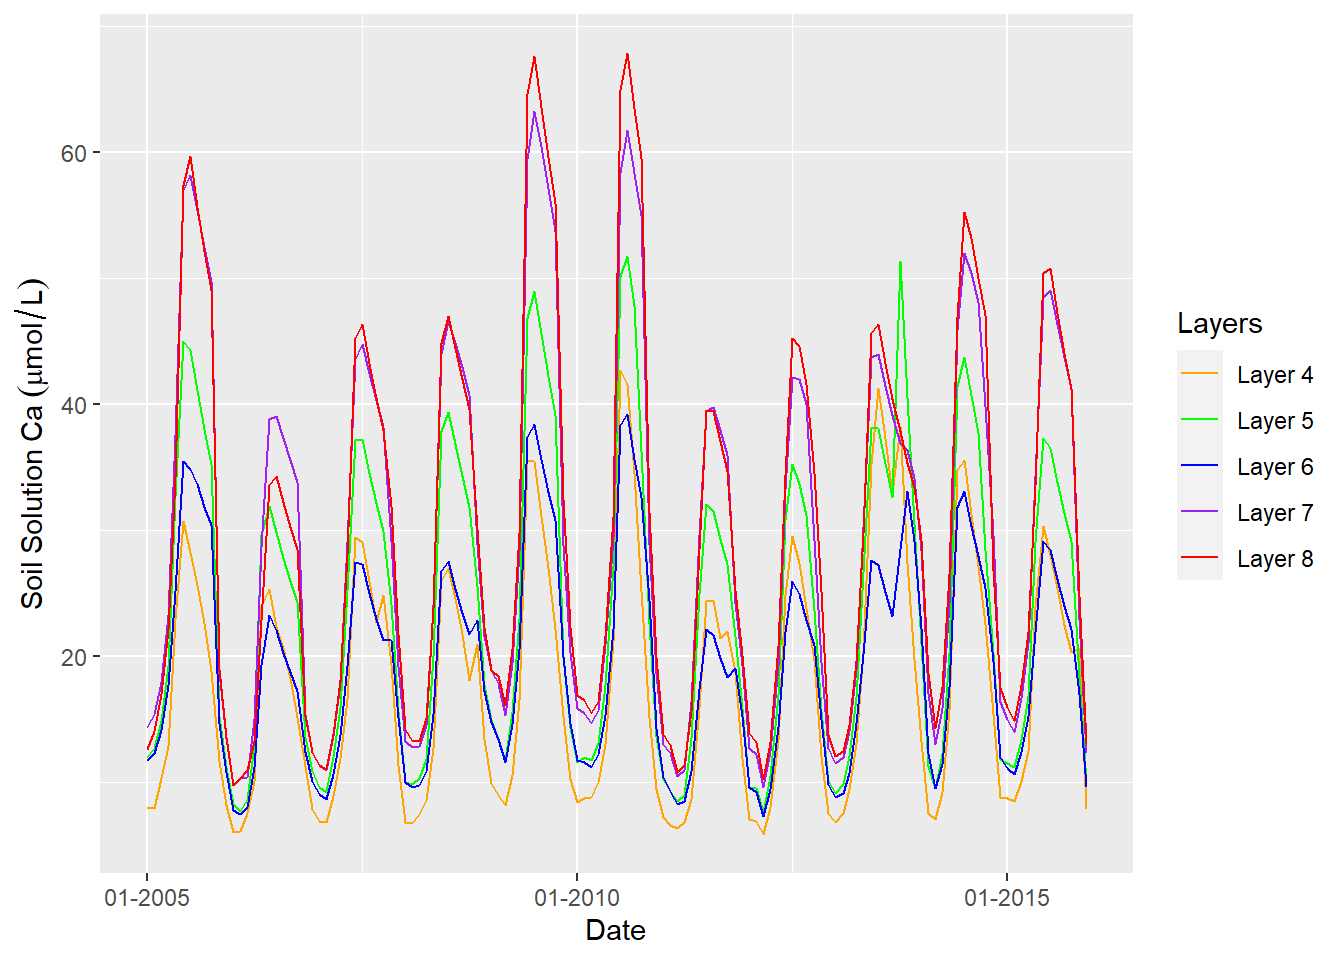
\includegraphics[width=0.5\linewidth]{Master_Report_files/figure-latex/figures-side-2} \caption{Figure 1: Monthly Calcium Concentrations by Soil Layer}\label{fig:figures-side}
\end{figure}
\begin{figure}[H]
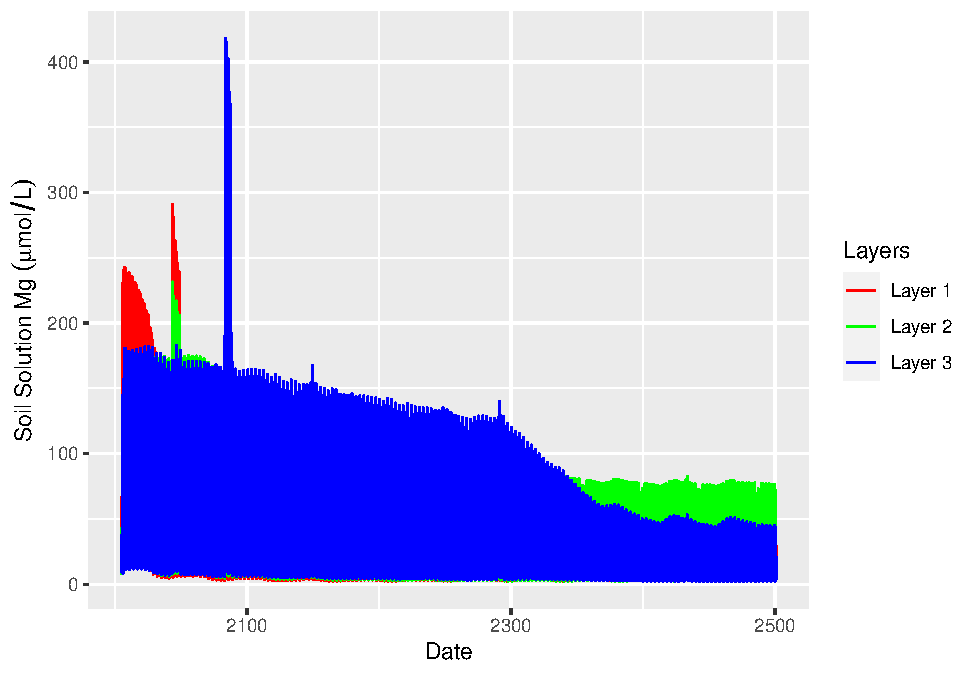
\includegraphics[width=0.5\linewidth]{Master_Report_files/figure-latex/unnamed-chunk-7-1} 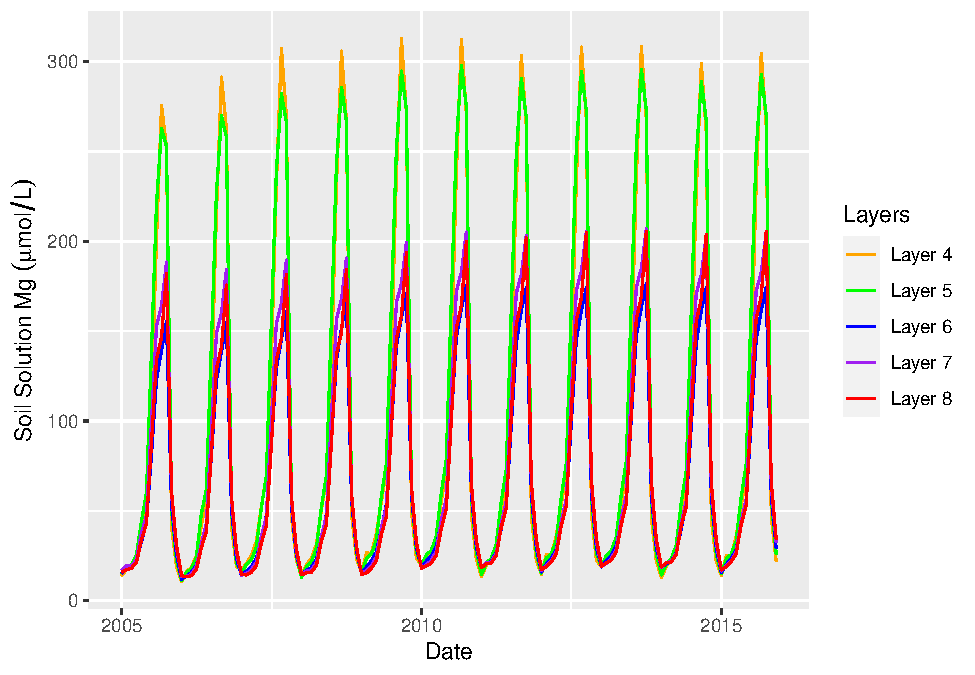
\includegraphics[width=0.5\linewidth]{Master_Report_files/figure-latex/unnamed-chunk-7-2} \caption{Figure 2: Monthly Magnesium Concentrations by Soil Layer}\label{fig:unnamed-chunk-7}
\end{figure}
\begin{figure}[H]
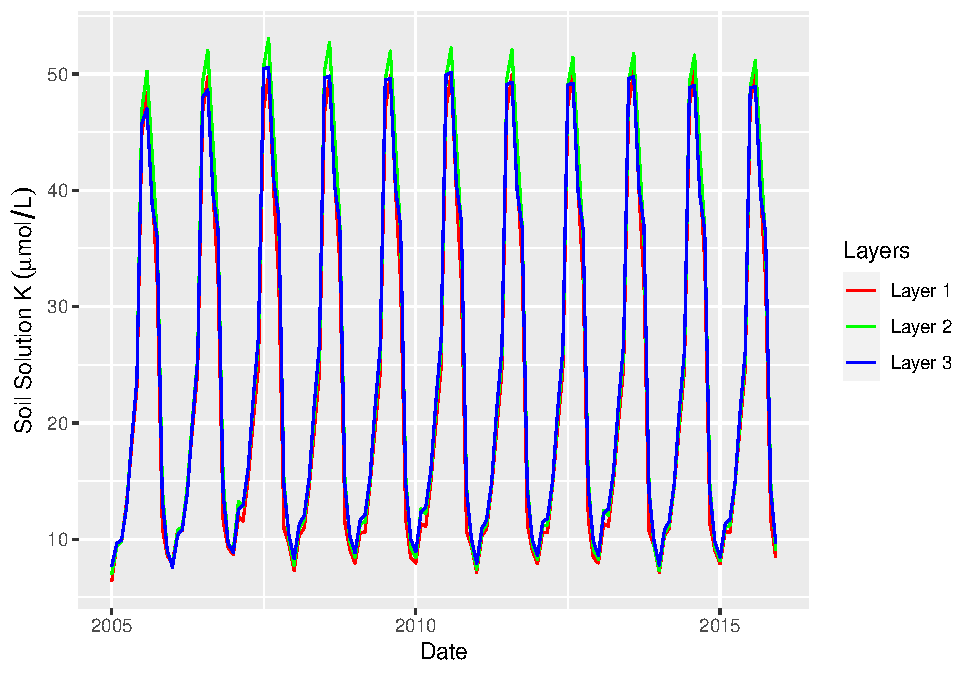
\includegraphics[width=0.5\linewidth]{Master_Report_files/figure-latex/unnamed-chunk-8-1} 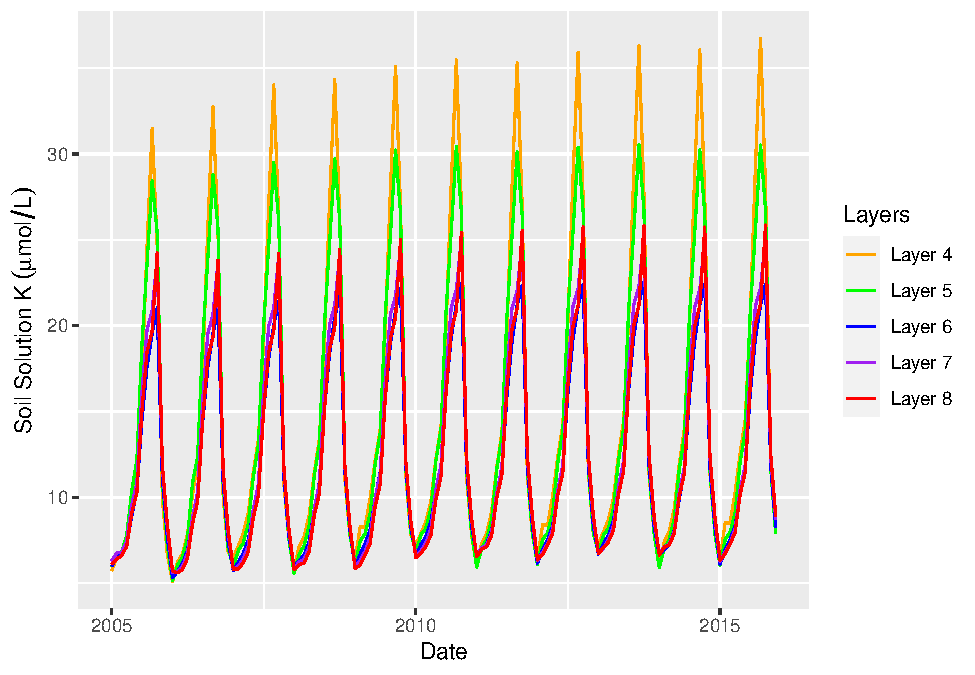
\includegraphics[width=0.5\linewidth]{Master_Report_files/figure-latex/unnamed-chunk-8-2} \caption{Figure 3: Monthly Potassium Concentrations by Soil Layer}\label{fig:unnamed-chunk-8}
\end{figure}
\begin{figure}[H]
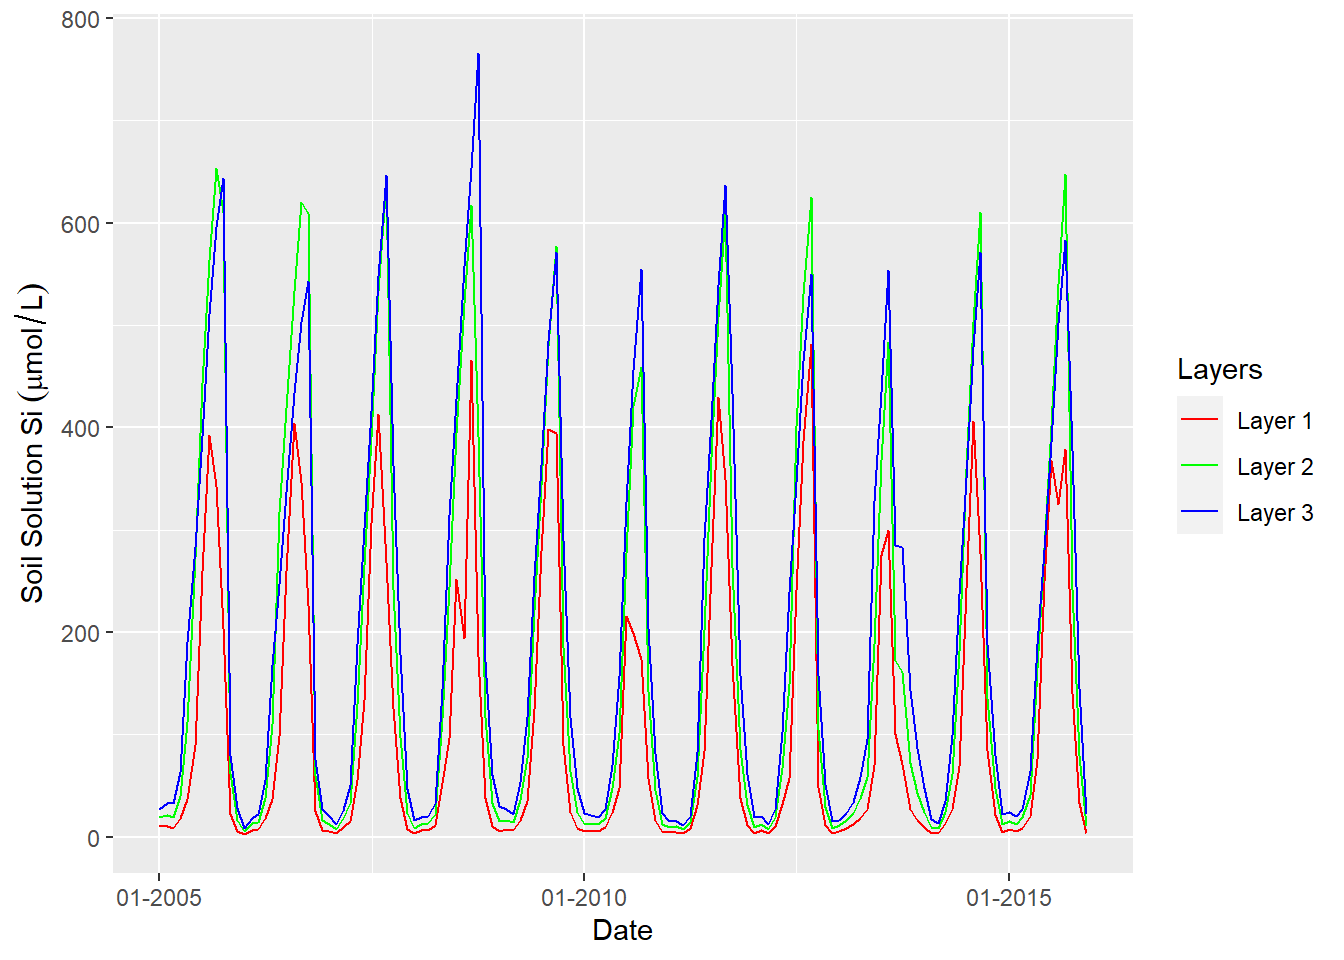
\includegraphics[width=0.5\linewidth]{Master_Report_files/figure-latex/unnamed-chunk-9-1} 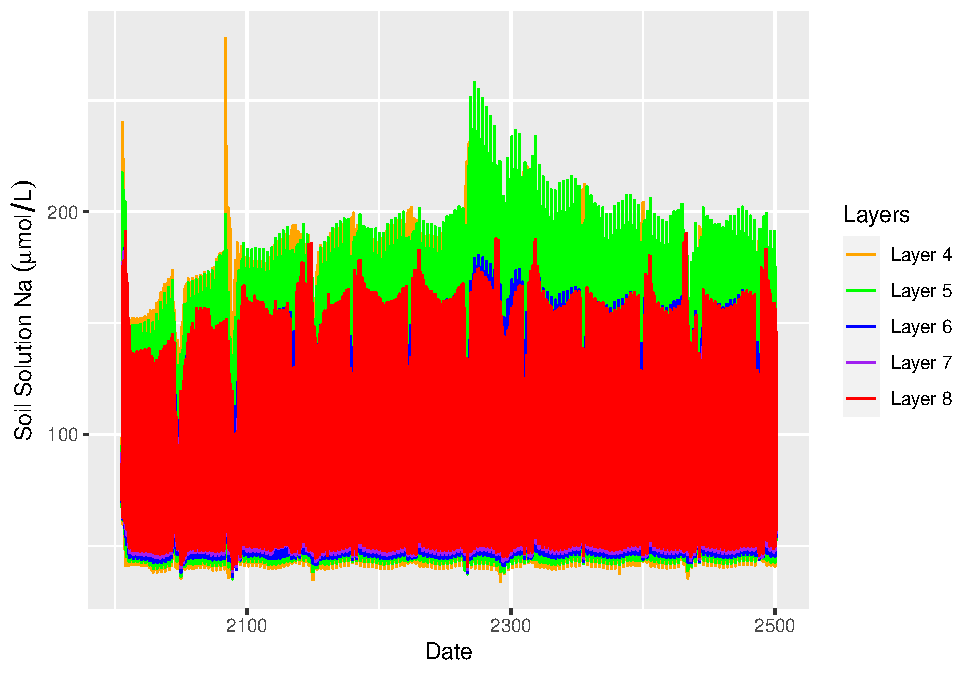
\includegraphics[width=0.5\linewidth]{Master_Report_files/figure-latex/unnamed-chunk-9-2} \caption{Figure 4: Monthly Sodium Concentrations by Soil Layer}\label{fig:unnamed-chunk-9}
\end{figure}

\begin{figure}[H]
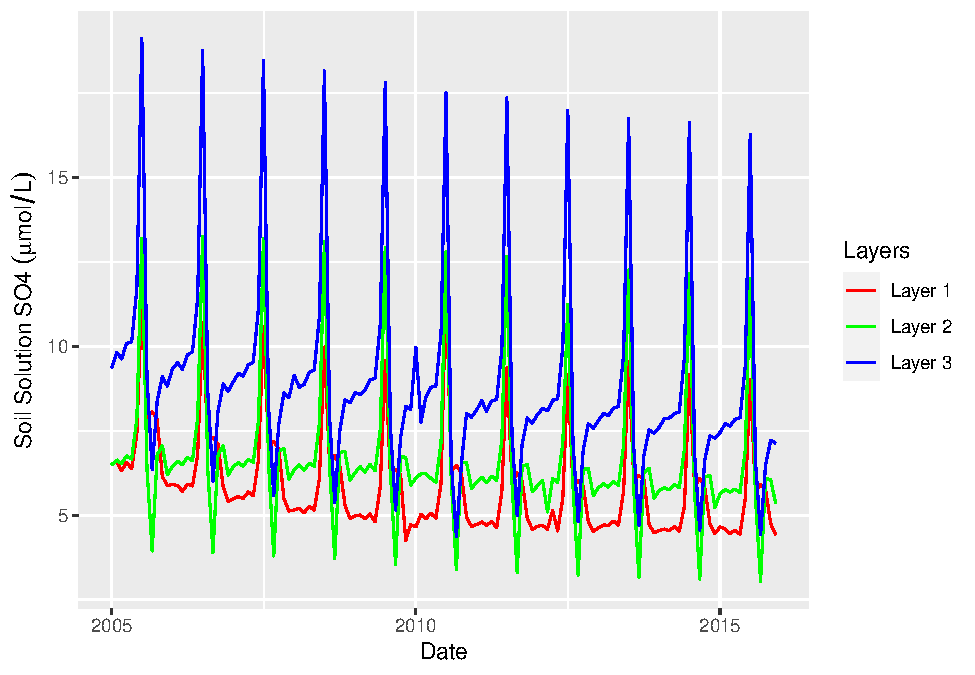
\includegraphics[width=0.5\linewidth]{Master_Report_files/figure-latex/unnamed-chunk-10-1} 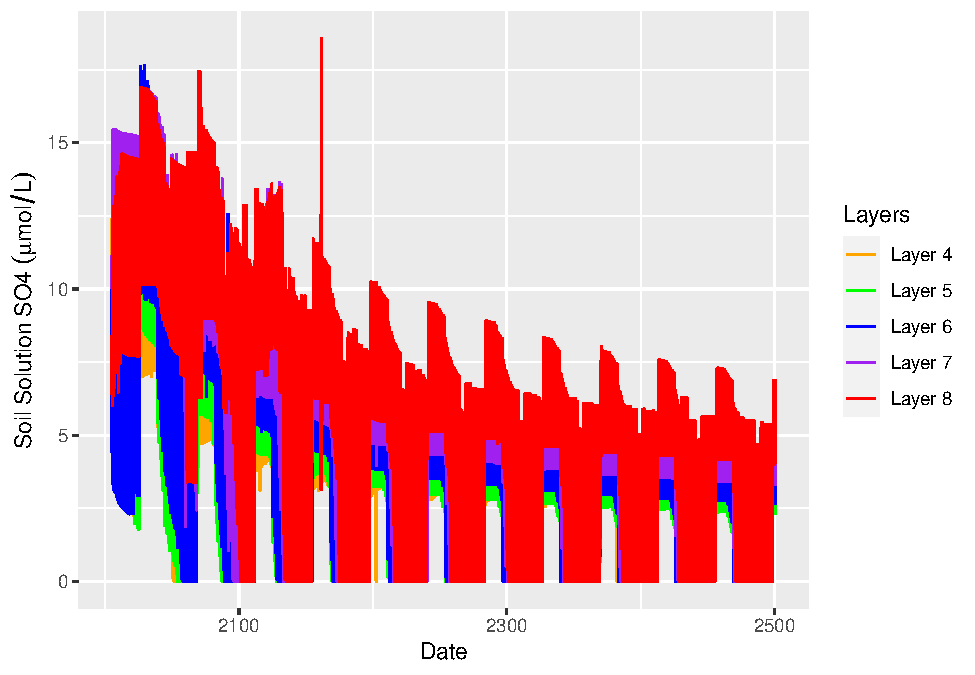
\includegraphics[width=0.5\linewidth]{Master_Report_files/figure-latex/unnamed-chunk-10-2} \caption{Figure 5: Monthly Aluminum Concentrations by Soil Layer}\label{fig:unnamed-chunk-10}
\end{figure}

\begin{figure}[H]
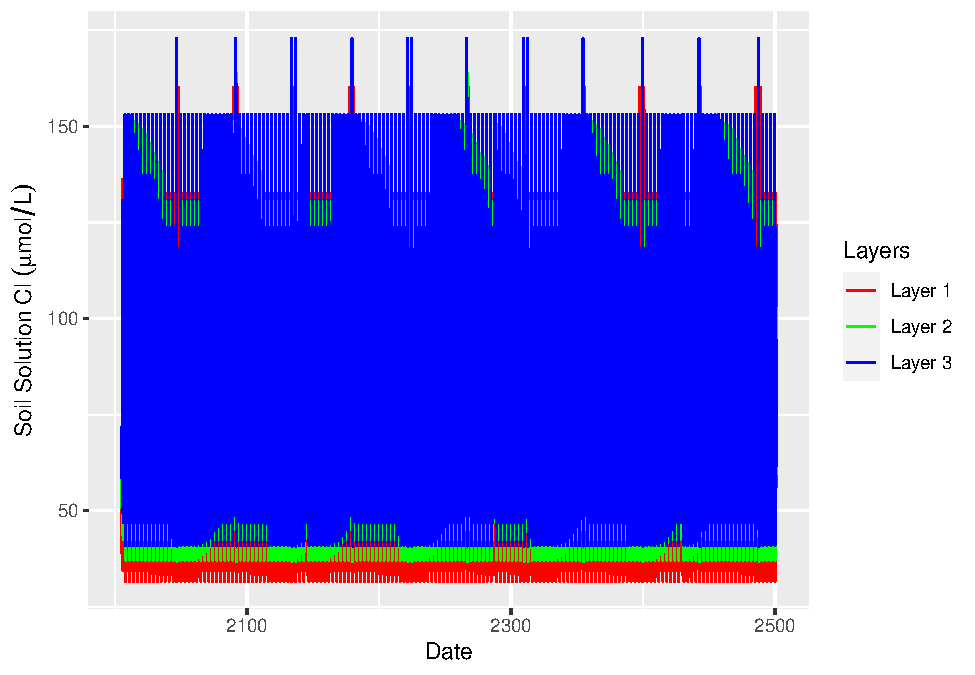
\includegraphics[width=0.5\linewidth]{Master_Report_files/figure-latex/unnamed-chunk-11-1} 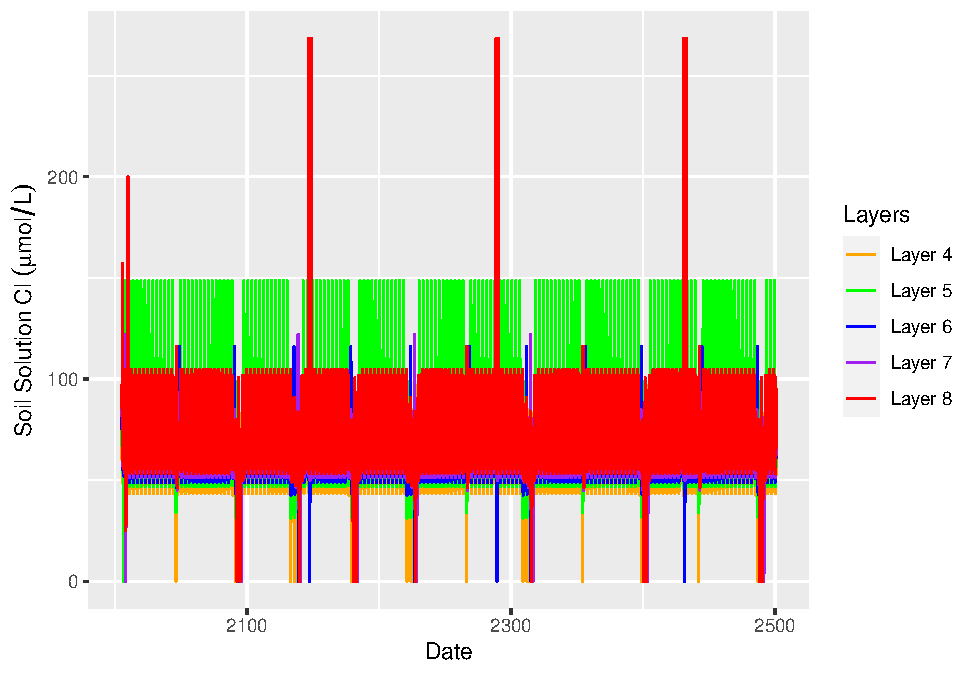
\includegraphics[width=0.5\linewidth]{Master_Report_files/figure-latex/unnamed-chunk-11-2} \caption{Figure 6: Monthly SiO2 Concentrations by Soil Layer}\label{fig:unnamed-chunk-11}
\end{figure}

\begin{figure}[H]
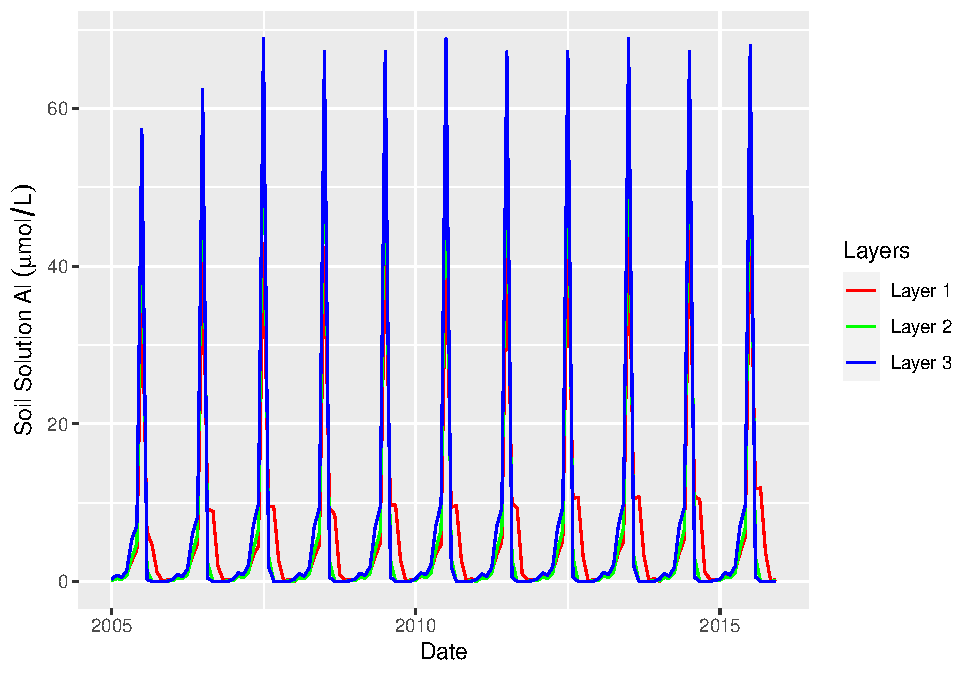
\includegraphics[width=0.5\linewidth]{Master_Report_files/figure-latex/unnamed-chunk-12-1} 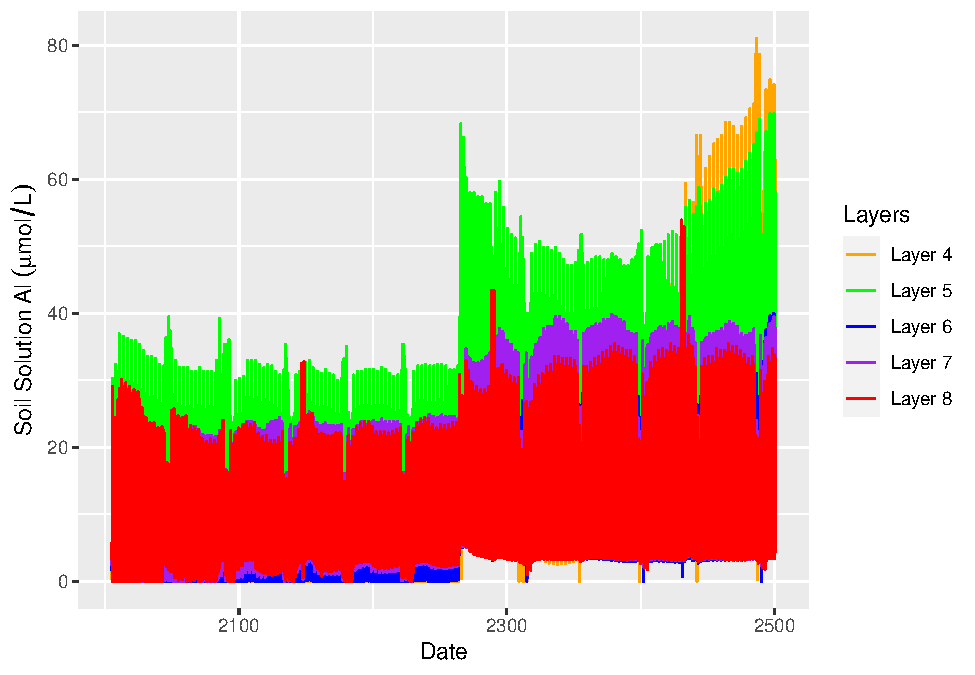
\includegraphics[width=0.5\linewidth]{Master_Report_files/figure-latex/unnamed-chunk-12-2} \caption{Figure 7: Monthly Organic Acid Base (R-) Concentrations by Soil Layer}\label{fig:unnamed-chunk-12}
\end{figure}

\begin{figure}[H]
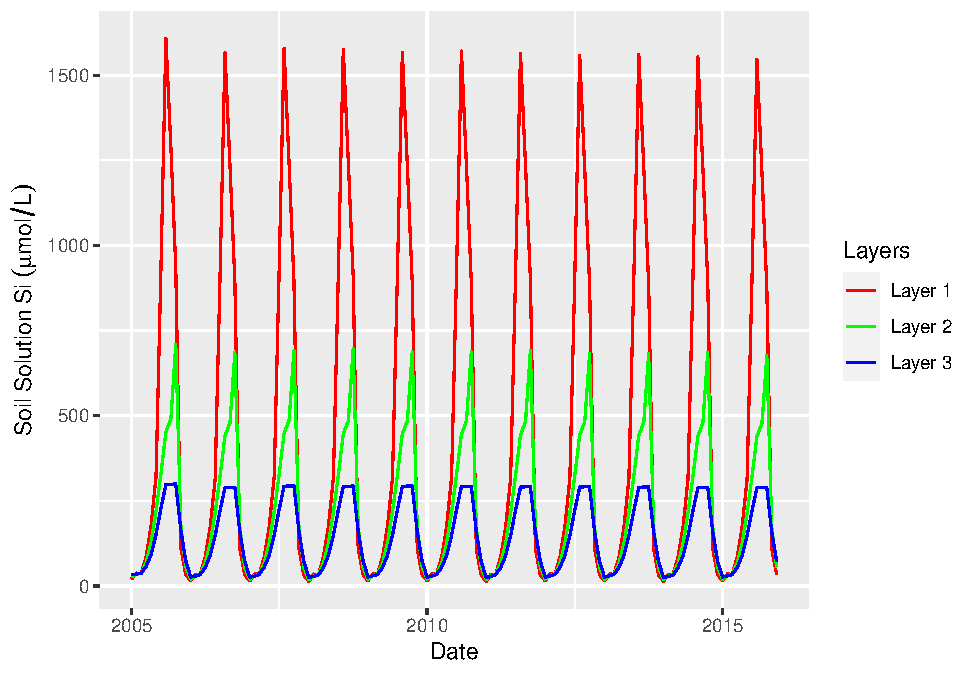
\includegraphics[width=0.5\linewidth]{Master_Report_files/figure-latex/unnamed-chunk-13-1} 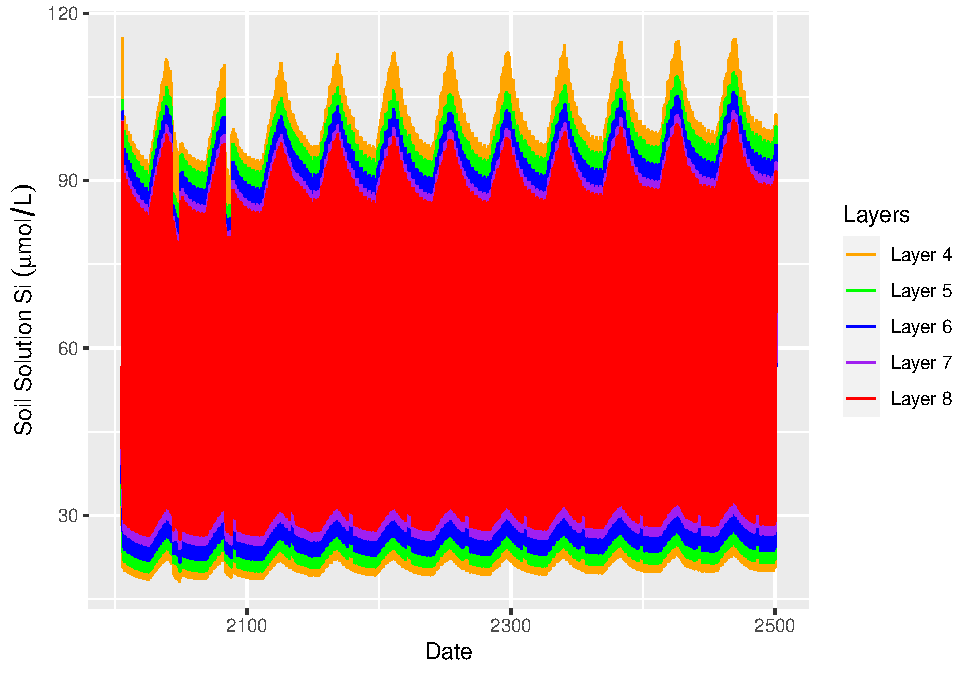
\includegraphics[width=0.5\linewidth]{Master_Report_files/figure-latex/unnamed-chunk-13-2} \caption{Figure 8: Monthly pH by Soil Layer}\label{fig:unnamed-chunk-13}
\end{figure}

\hypertarget{weathering-results}{%
\subsubsection{Weathering Results}\label{weathering-results}}

\hypertarget{figures}{%
\paragraph{Figures}\label{figures}}

\begin{figure}[H]
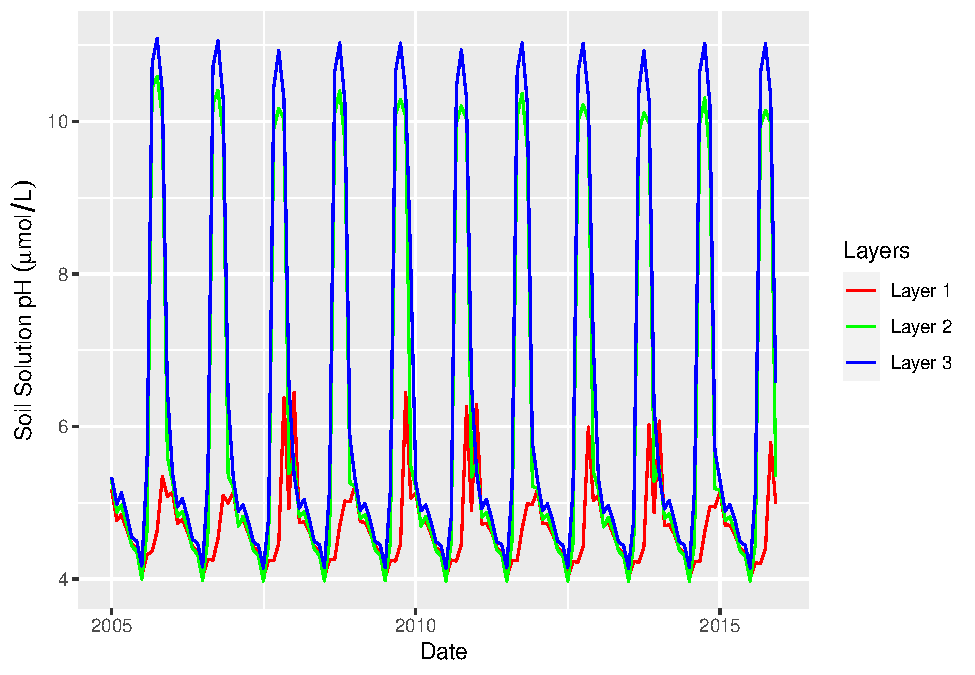
\includegraphics[width=0.5\linewidth]{Master_Report_files/figure-latex/unnamed-chunk-15-1} 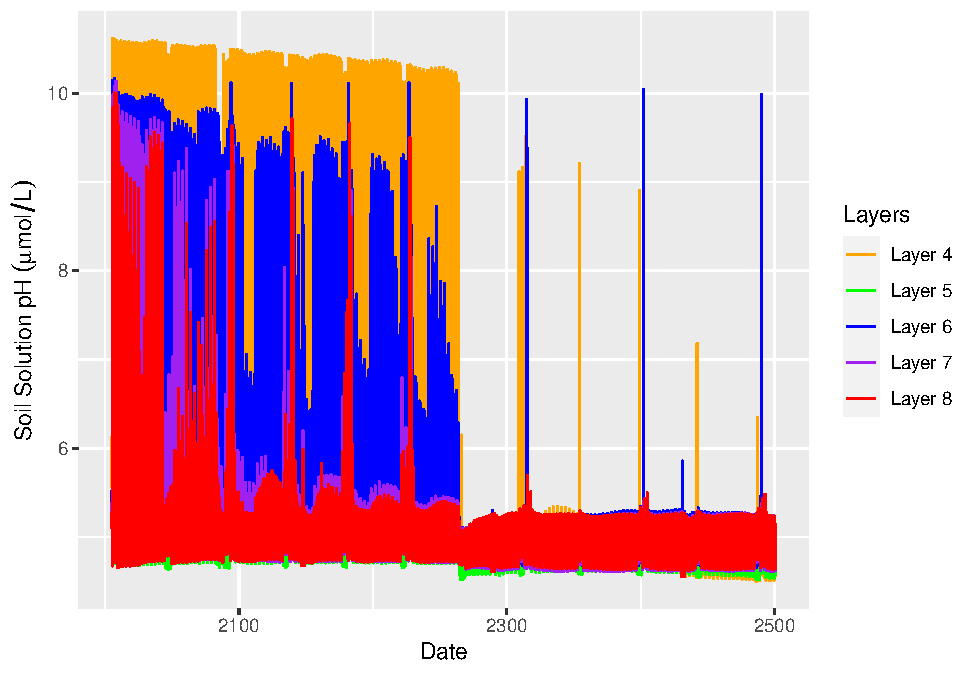
\includegraphics[width=0.5\linewidth]{Master_Report_files/figure-latex/unnamed-chunk-15-2} \caption{Figure 9: Calcium Weathering by Layer}\label{fig:unnamed-chunk-15}
\end{figure}

\begin{figure}[H]
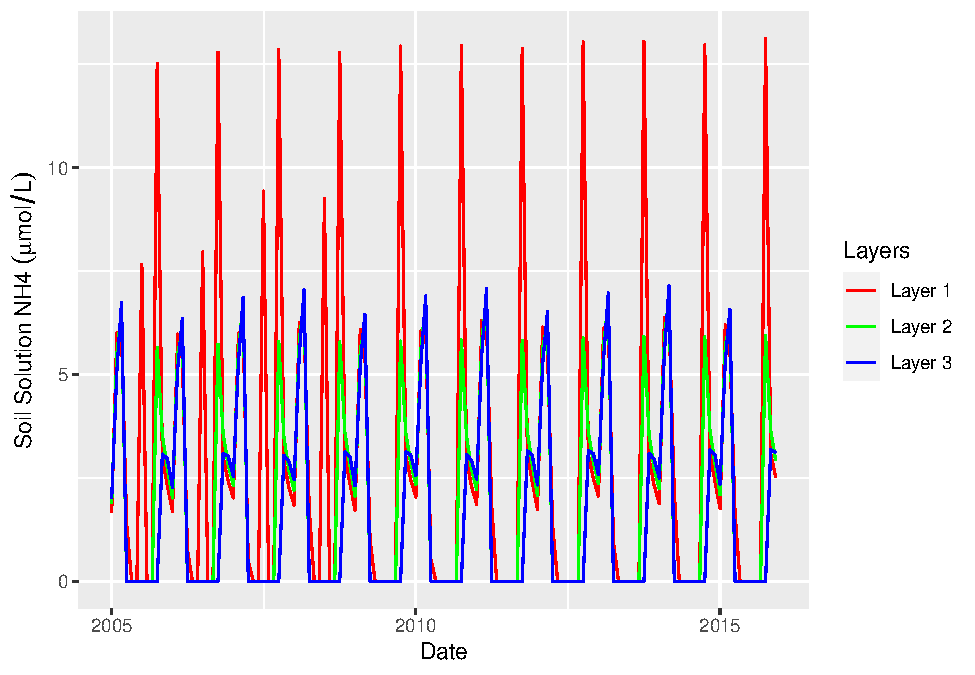
\includegraphics[width=0.5\linewidth]{Master_Report_files/figure-latex/unnamed-chunk-16-1} 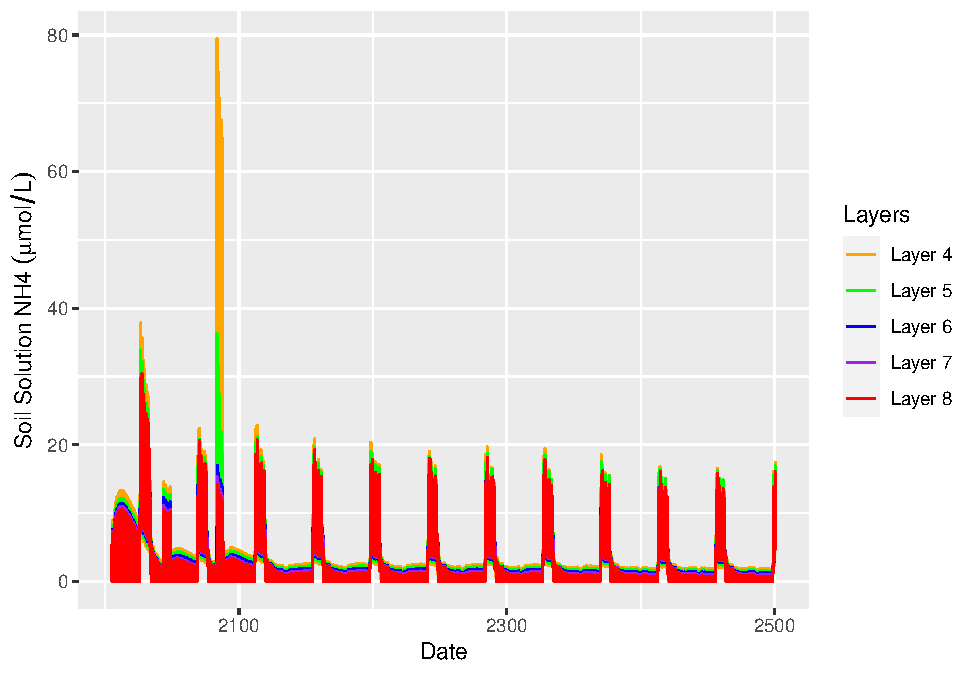
\includegraphics[width=0.5\linewidth]{Master_Report_files/figure-latex/unnamed-chunk-16-2} \caption{Figure 10: Magnesium Weathering by Layer}\label{fig:unnamed-chunk-16}
\end{figure}

\begin{figure}[H]
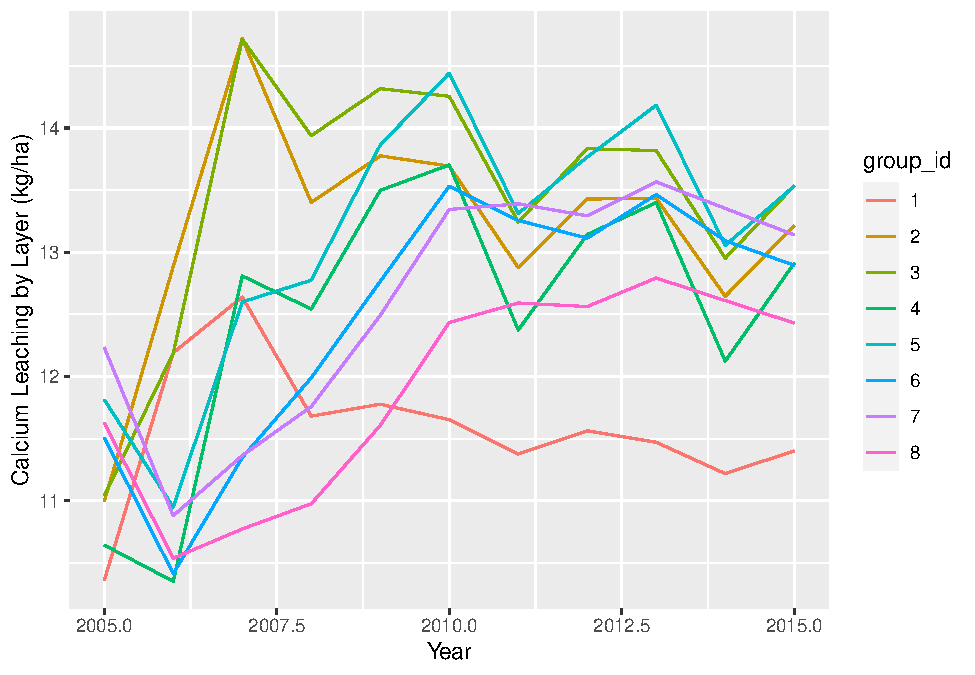
\includegraphics[width=0.5\linewidth]{Master_Report_files/figure-latex/unnamed-chunk-18-1} 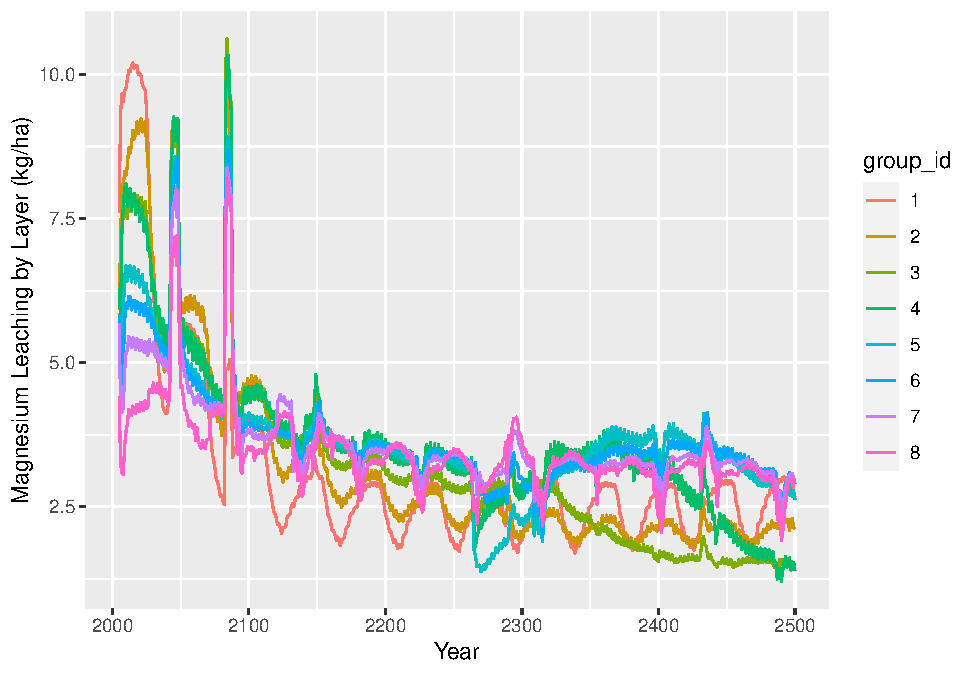
\includegraphics[width=0.5\linewidth]{Master_Report_files/figure-latex/unnamed-chunk-18-2} \caption{Figure 12: Aluminum Weathering by Layer}\label{fig:unnamed-chunk-18}
\end{figure}

\begin{figure}[H]
\includegraphics[width=0.5\linewidth]{Master_Report_files/figure-latex/unnamed-chunk-19-1} \includegraphics[width=0.5\linewidth]{Master_Report_files/figure-latex/unnamed-chunk-19-2} \caption{Figure 13: Phosphate Weathering by Layer}\label{fig:unnamed-chunk-19}
\end{figure}

\begin{figure}[H]
\includegraphics[width=0.5\linewidth]{Master_Report_files/figure-latex/unnamed-chunk-20-1} \includegraphics[width=0.5\linewidth]{Master_Report_files/figure-latex/unnamed-chunk-20-2} \caption{Figure 14: Silica Weathering by Layer}\label{fig:unnamed-chunk-20}
\end{figure}

\begin{figure}[H]
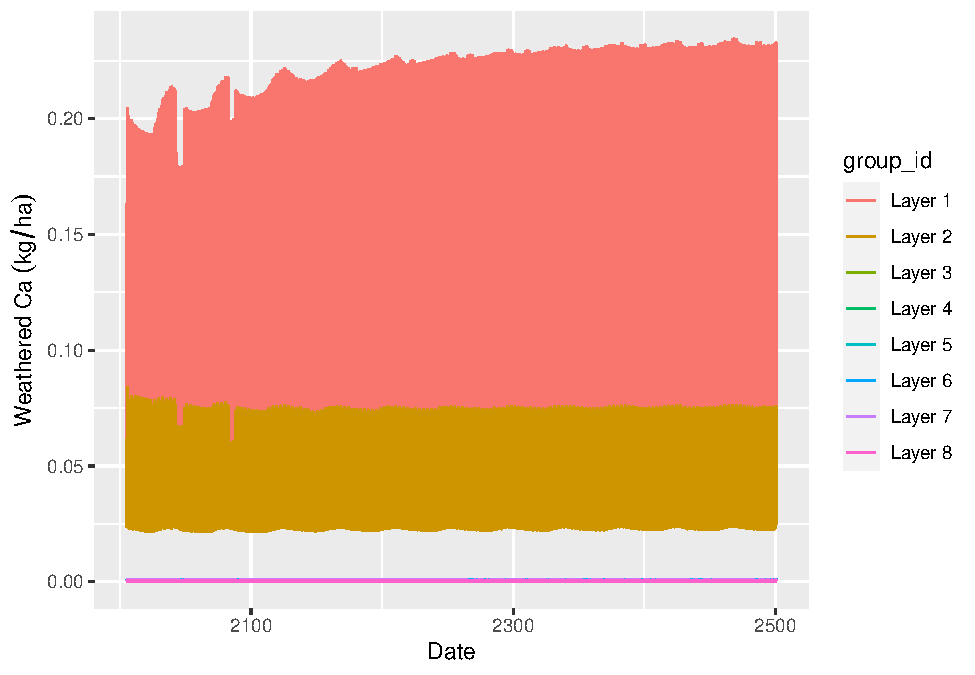
\includegraphics[width=0.5\linewidth]{Master_Report_files/figure-latex/unnamed-chunk-21-1} \includegraphics[width=0.5\linewidth]{Master_Report_files/figure-latex/unnamed-chunk-21-2} \caption{Figure 15: Sodium Weathering by Layer}\label{fig:unnamed-chunk-21}
\end{figure}

\hypertarget{litter-pool-results}{%
\subsubsection{Litter Pool Results}\label{litter-pool-results}}

\begin{figure}[H]
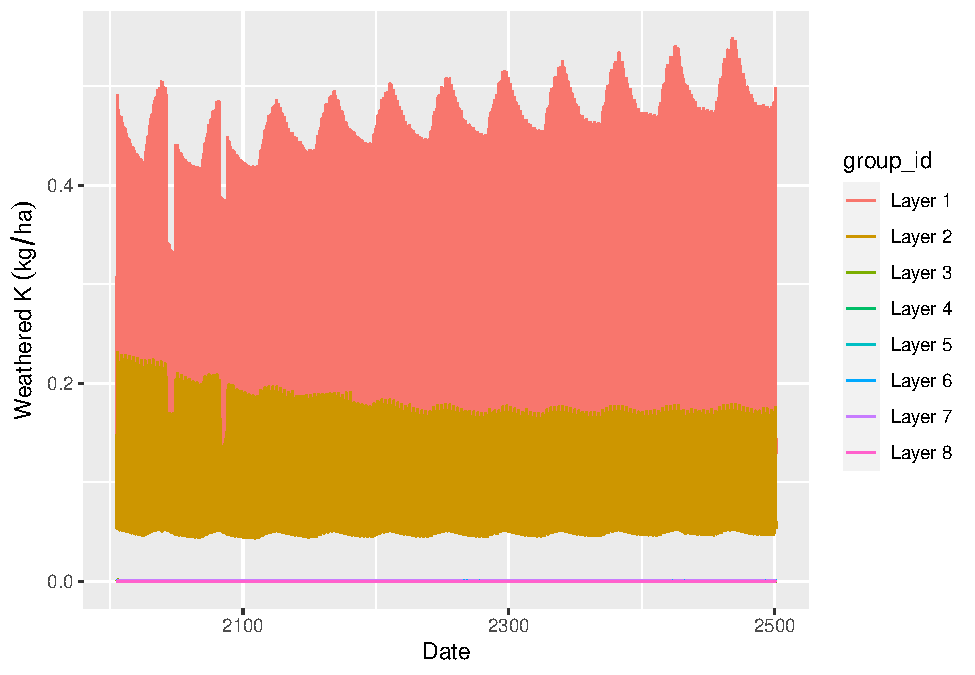
\includegraphics[width=0.5\linewidth]{Master_Report_files/figure-latex/unnamed-chunk-23-1} \caption{Figure 17: Litter Pool Carbon Content Over Simulation Period}\label{fig:unnamed-chunk-23}
\end{figure}

\begin{figure}[H]
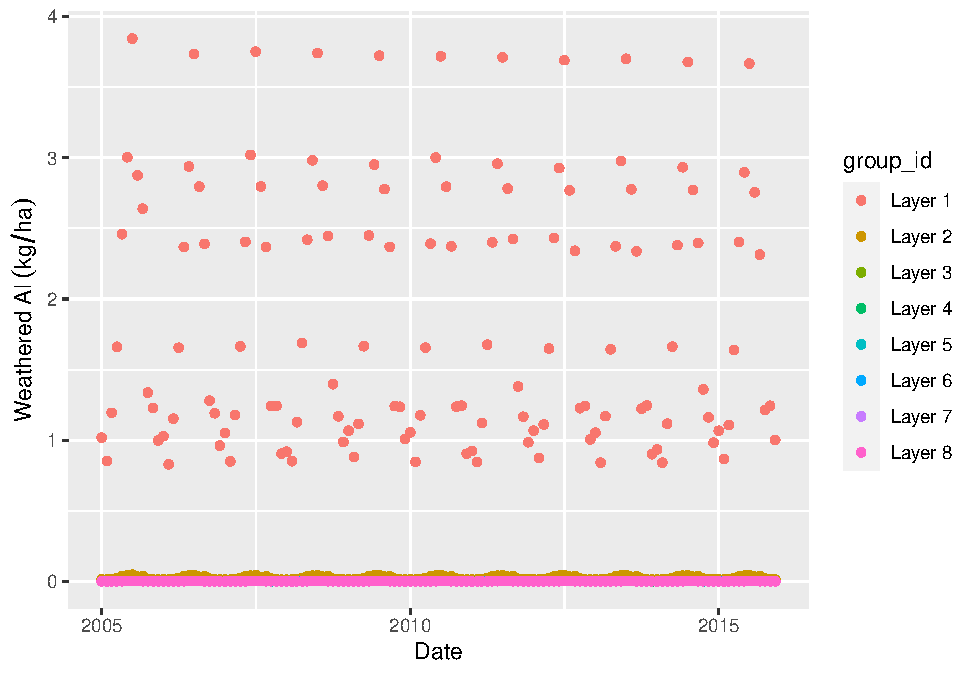
\includegraphics[width=0.5\linewidth]{Master_Report_files/figure-latex/unnamed-chunk-24-1} \caption{Figure 18: Litter Pool Ca Content Over Simulation Period}\label{fig:unnamed-chunk-24}
\end{figure}

\begin{figure}[H]
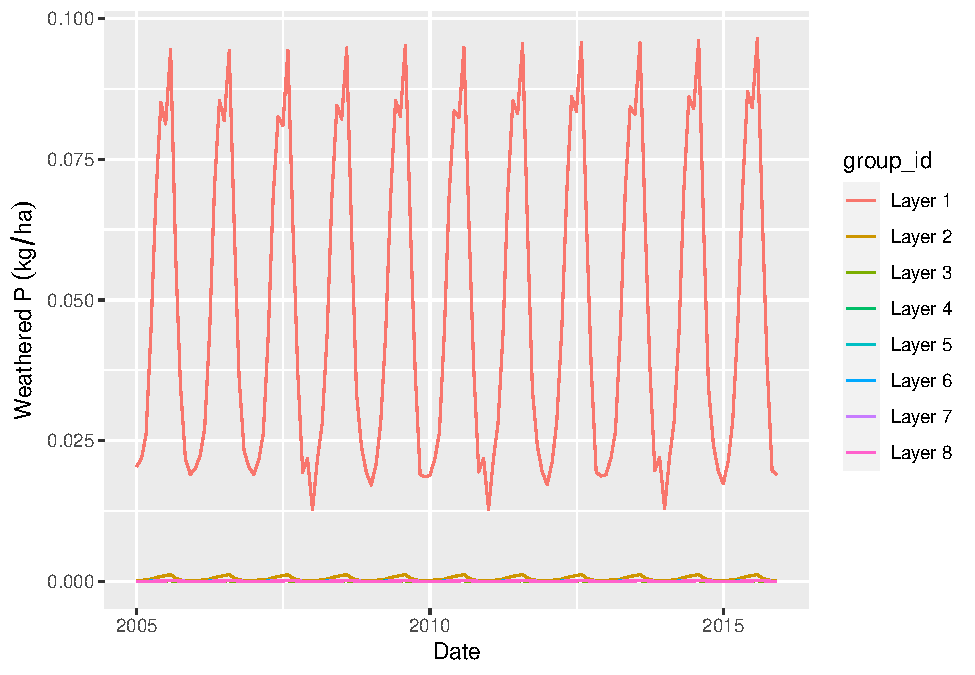
\includegraphics[width=0.5\linewidth]{Master_Report_files/figure-latex/unnamed-chunk-25-1} \caption{Figure 19: Litter Pool Mg Content Over Simulation Period}\label{fig:unnamed-chunk-25}
\end{figure}

\begin{figure}[H]
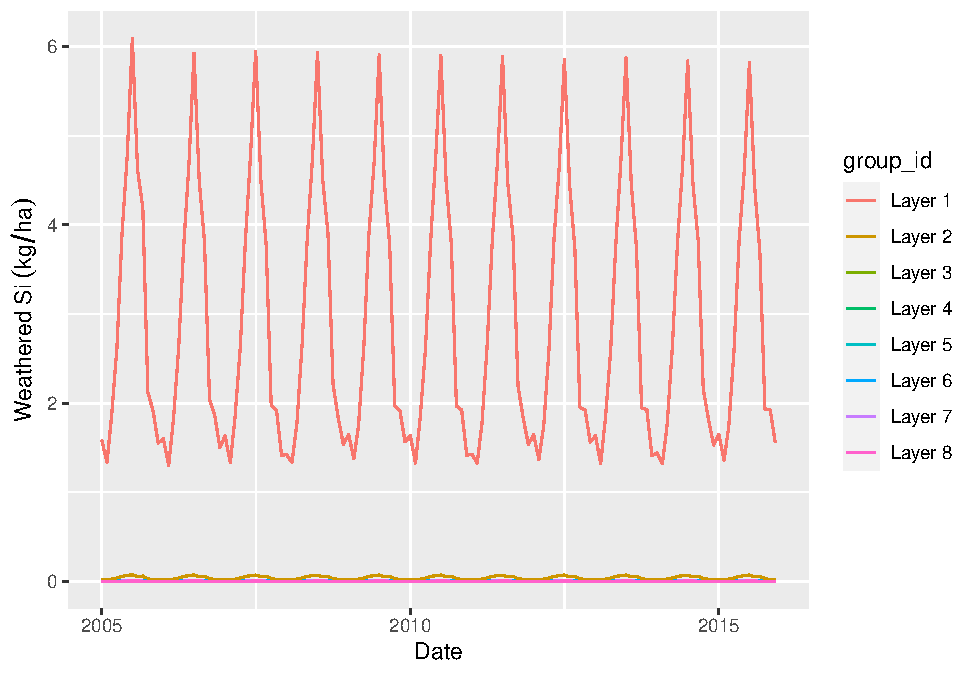
\includegraphics[width=0.5\linewidth]{Master_Report_files/figure-latex/unnamed-chunk-26-1} \caption{Figure 20: Litter Pool K Content Over Simulation Period}\label{fig:unnamed-chunk-26}
\end{figure}

\begin{figure}[H]
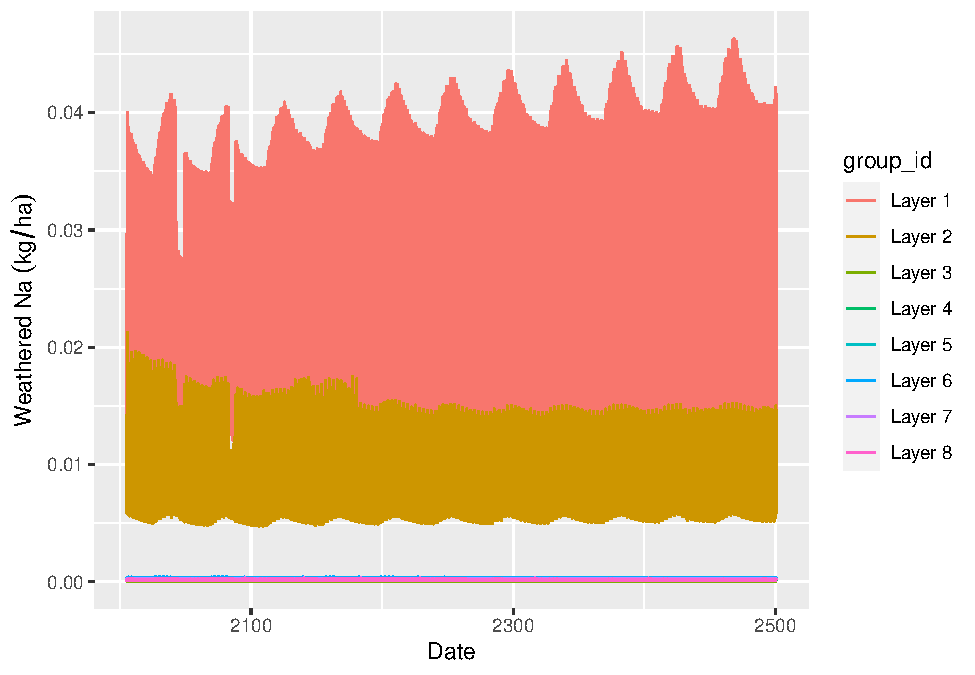
\includegraphics[width=0.5\linewidth]{Master_Report_files/figure-latex/unnamed-chunk-27-1} \caption{Figure 21: Litter Pool P Content Over Simulation Period}\label{fig:unnamed-chunk-27}
\end{figure}

\begin{figure}[H]
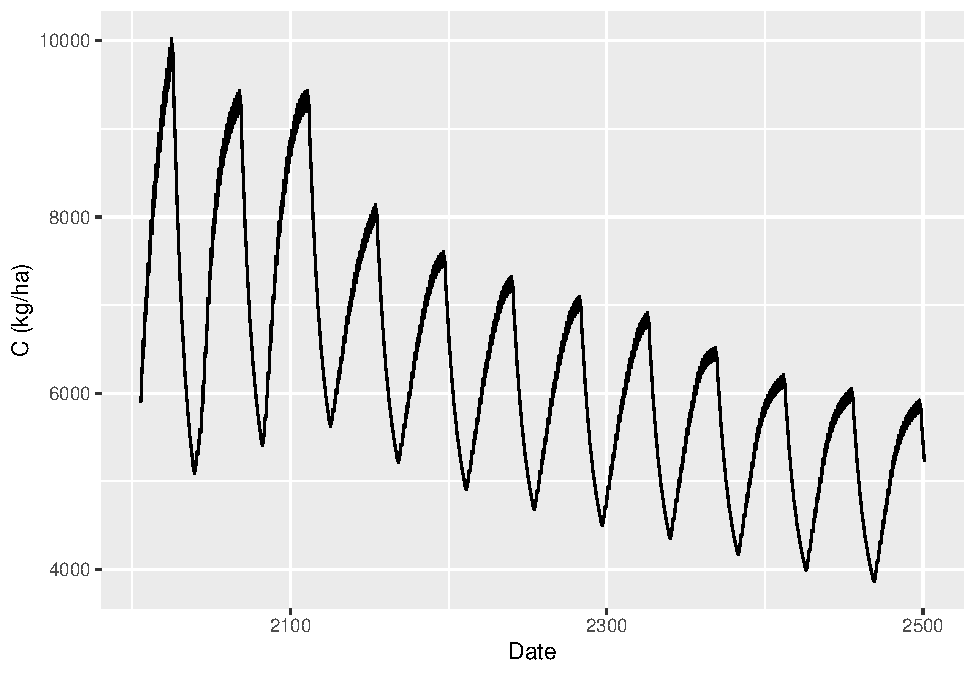
\includegraphics[width=0.5\linewidth]{Master_Report_files/figure-latex/unnamed-chunk-28-1} \caption{Figure 22: Litter Pool S Content Over Simulation Period}\label{fig:unnamed-chunk-28}
\end{figure}

\hypertarget{tree-nutrient-content}{%
\subsubsection{Tree Nutrient Content}\label{tree-nutrient-content}}

\begin{figure}[H]

{\centering \subfloat[Calcium content in each biomass compartment\label{fig:unnamed-chunk-29-1}]{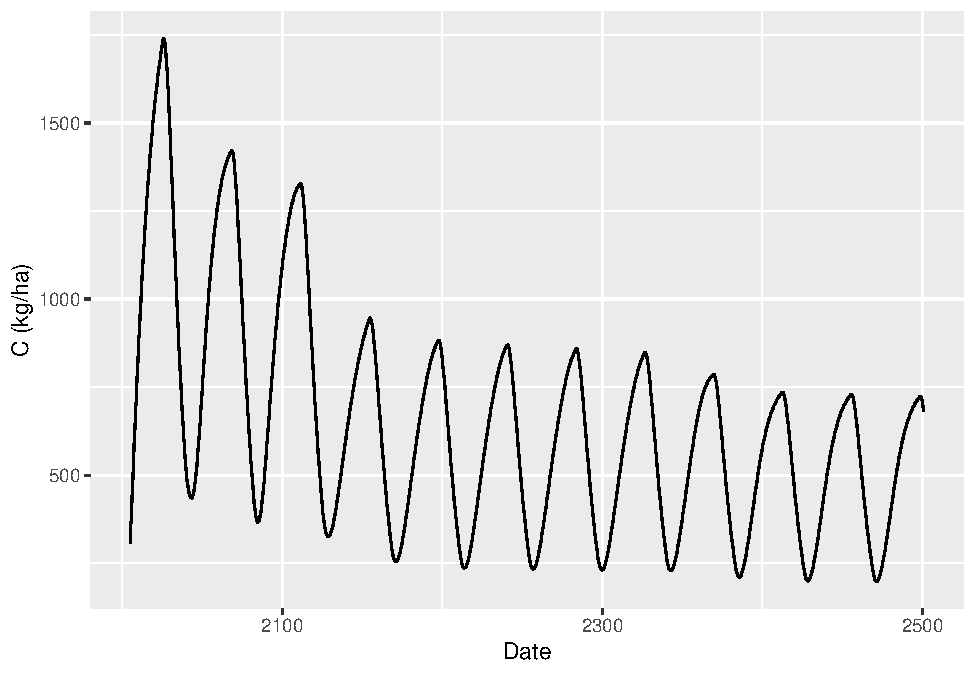
\includegraphics[width=0.5\linewidth]{Master_Report_files/figure-latex/unnamed-chunk-29-1} }\subfloat[Magnesium content in each biomass compartment\label{fig:unnamed-chunk-29-2}]{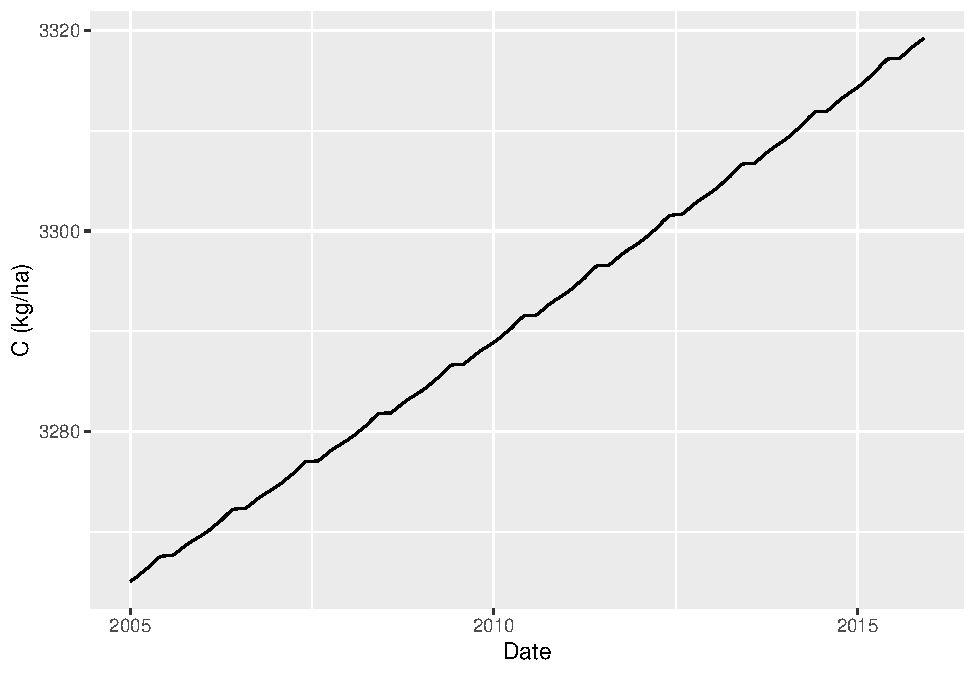
\includegraphics[width=0.5\linewidth]{Master_Report_files/figure-latex/unnamed-chunk-29-2} }\newline\subfloat[Potassium content in each biomass compartment\label{fig:unnamed-chunk-29-3}]{\includegraphics[width=0.5\linewidth]{Master_Report_files/figure-latex/unnamed-chunk-29-3} }

}

\caption{Base Cation Nutrient Content in Simulated Forest}\label{fig:unnamed-chunk-29}
\end{figure}

\begin{figure}[H]

{\centering \subfloat[Nitrogen content in each biomass compartment\label{fig:unnamed-chunk-30-1}]{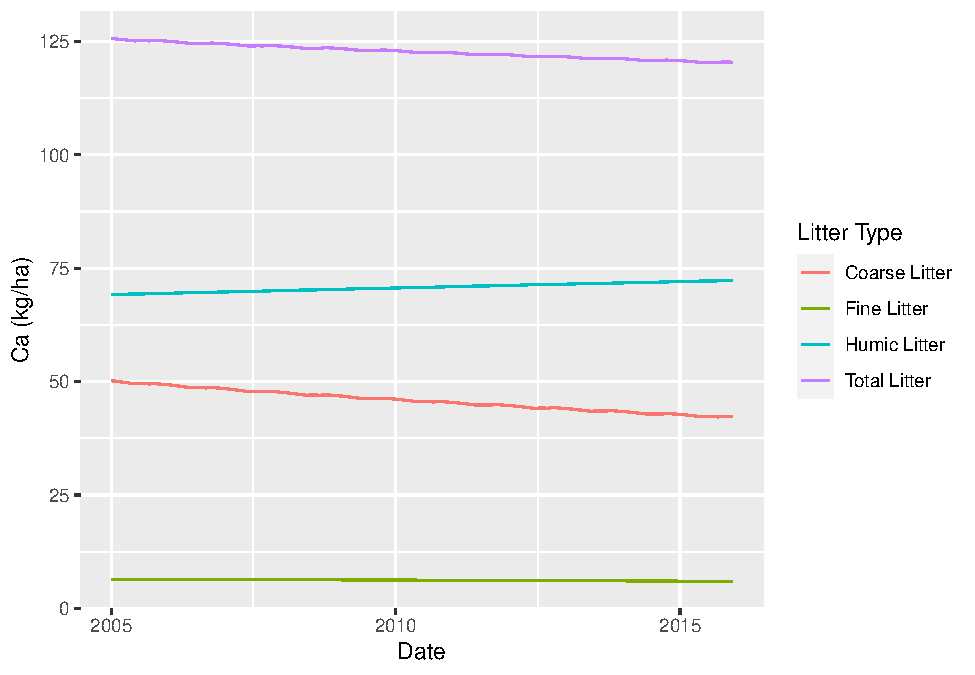
\includegraphics[width=0.5\linewidth]{Master_Report_files/figure-latex/unnamed-chunk-30-1} }\subfloat[Sulfur content in each biomass compartment\label{fig:unnamed-chunk-30-2}]{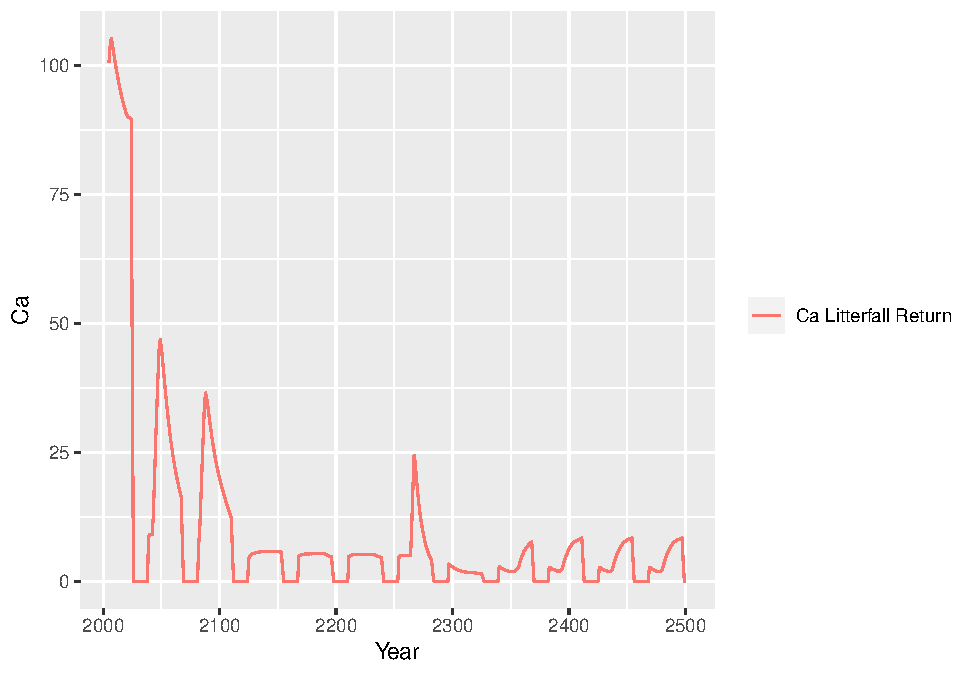
\includegraphics[width=0.5\linewidth]{Master_Report_files/figure-latex/unnamed-chunk-30-2} }\newline\subfloat[Phosphorous content in each biomass compartment\label{fig:unnamed-chunk-30-3}]{\includegraphics[width=0.5\linewidth]{Master_Report_files/figure-latex/unnamed-chunk-30-3} }\subfloat[Biomass of each compartment\label{fig:unnamed-chunk-30-4}]{\includegraphics[width=0.5\linewidth]{Master_Report_files/figure-latex/unnamed-chunk-30-4} }

}

\caption{N, S, and P Nutrient Contents and biomass per compartment}\label{fig:unnamed-chunk-30}
\end{figure}

\#\#\# Comparison of Inputs and Outputs

\begin{figure}[H]

{\centering \subfloat[Ca Leaching Losses\label{fig:unnamed-chunk-32-1}]{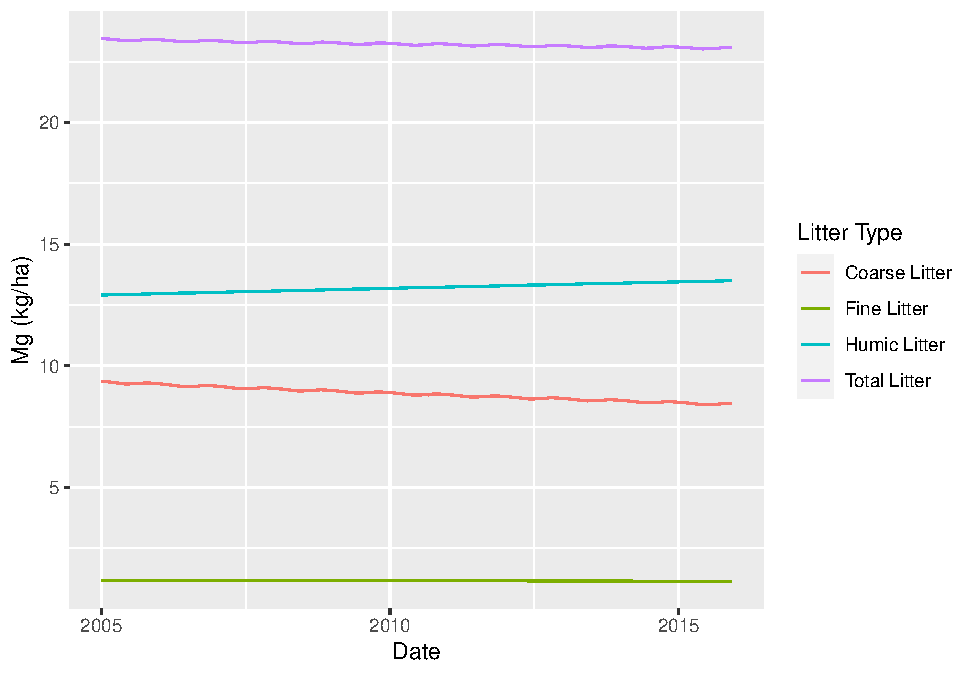
\includegraphics[width=0.5\linewidth]{Master_Report_files/figure-latex/unnamed-chunk-32-1} }\subfloat[Mg Leaching Losses\label{fig:unnamed-chunk-32-2}]{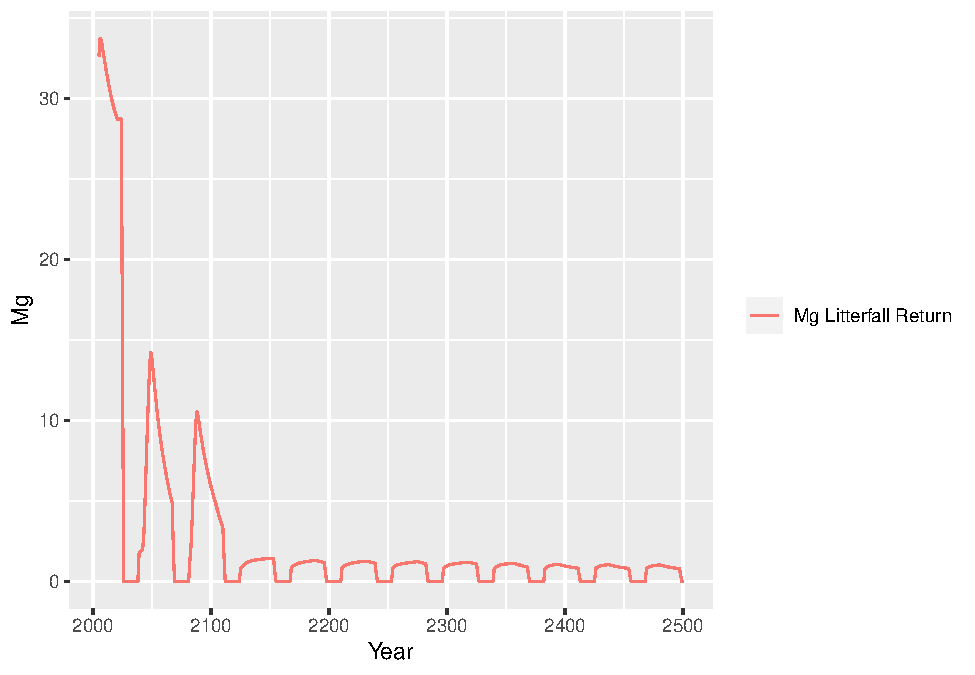
\includegraphics[width=0.5\linewidth]{Master_Report_files/figure-latex/unnamed-chunk-32-2} }

}

\caption{Annual Leaching Losses of Divalent Base Cations}\label{fig:unnamed-chunk-32}
\end{figure}

\begin{figure}[H]

{\centering \subfloat[K Leaching Losses\label{fig:unnamed-chunk-33-1}]{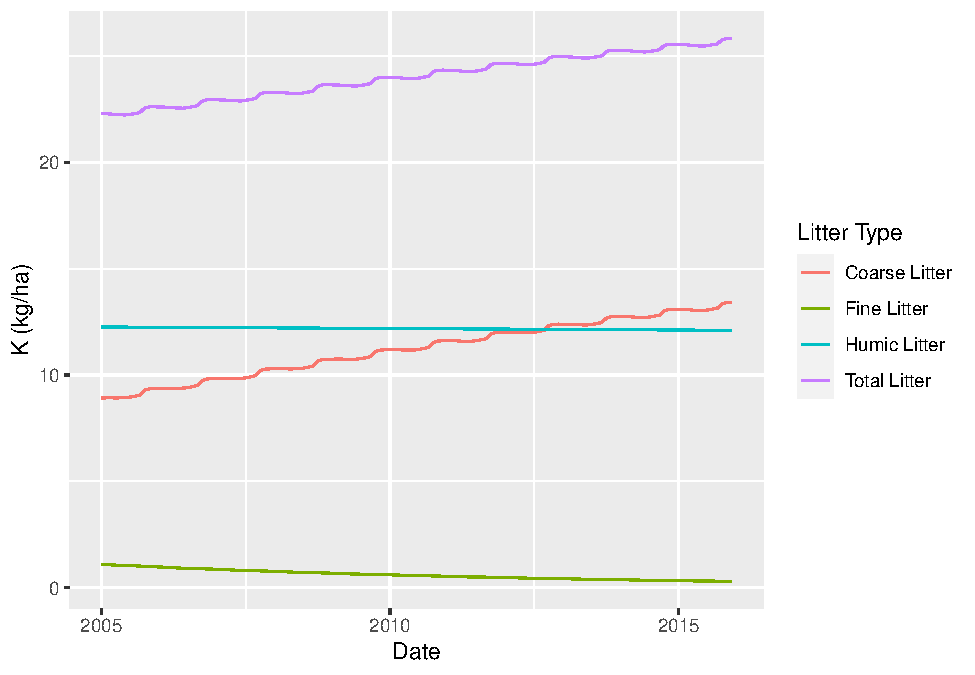
\includegraphics[width=0.5\linewidth]{Master_Report_files/figure-latex/unnamed-chunk-33-1} }\subfloat[Na Leaching Losses\label{fig:unnamed-chunk-33-2}]{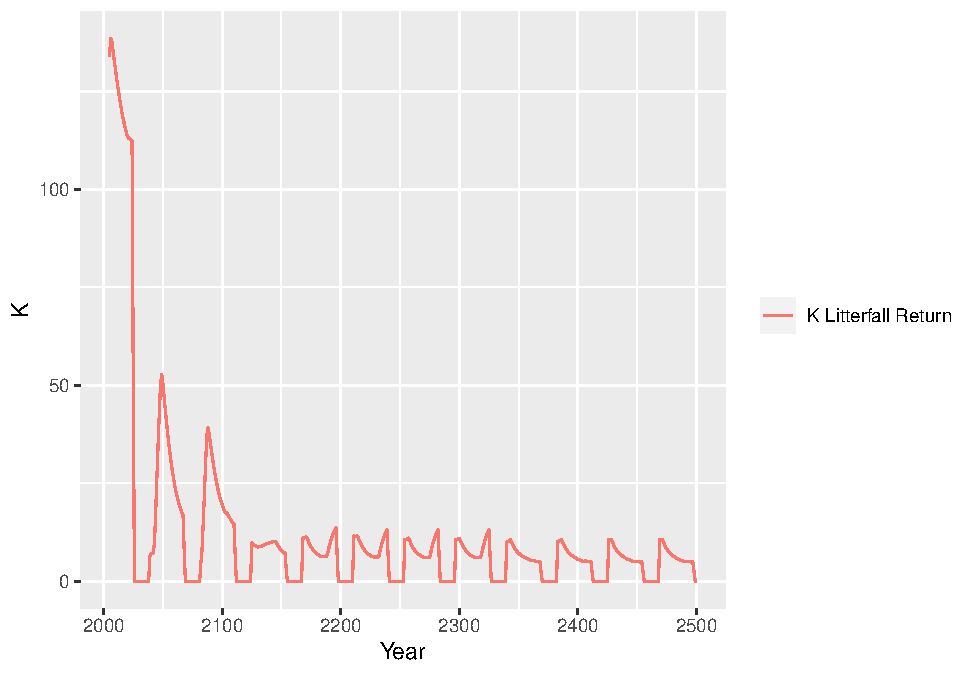
\includegraphics[width=0.5\linewidth]{Master_Report_files/figure-latex/unnamed-chunk-33-2} }

}

\caption{Annual Leaching Losses of Monovalent Base Cations}\label{fig:unnamed-chunk-33}
\end{figure}

\begin{figure}[H]

{\centering \subfloat[N Leaching Losses\label{fig:unnamed-chunk-34-1}]{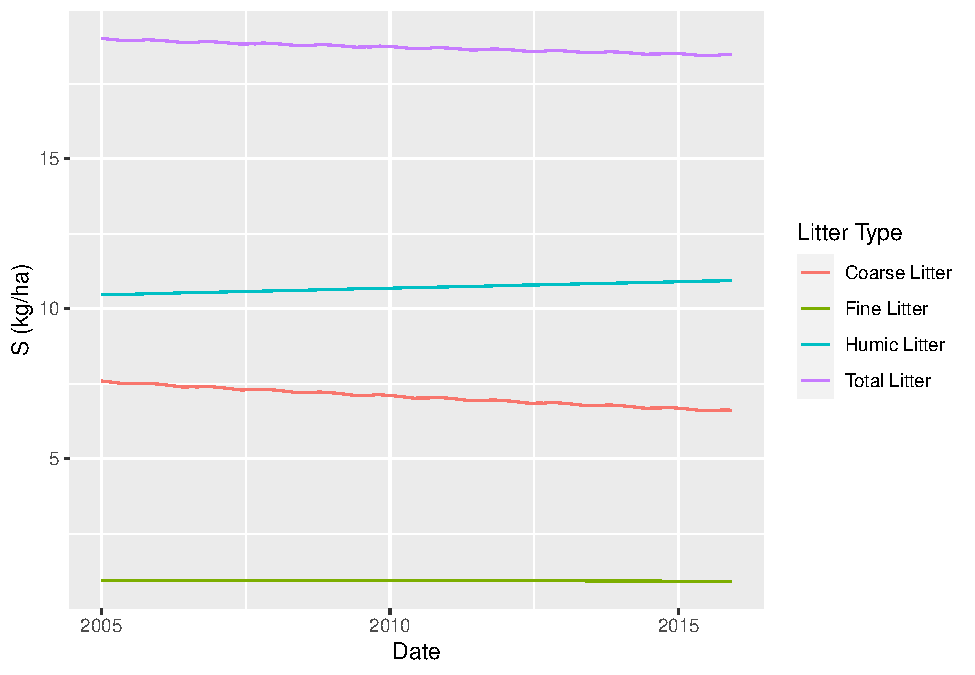
\includegraphics[width=0.5\linewidth]{Master_Report_files/figure-latex/unnamed-chunk-34-1} }\subfloat[S Leaching Losses\label{fig:unnamed-chunk-34-2}]{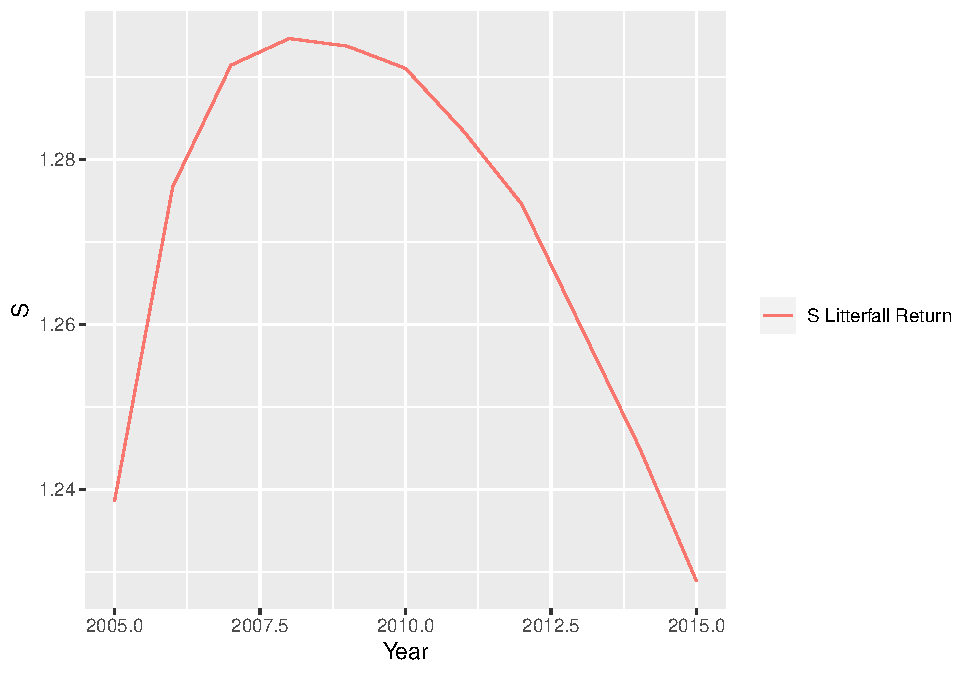
\includegraphics[width=0.5\linewidth]{Master_Report_files/figure-latex/unnamed-chunk-34-2} }\newline\subfloat[P Leaching Losses\label{fig:unnamed-chunk-34-3}]{\includegraphics[width=0.5\linewidth]{Master_Report_files/figure-latex/unnamed-chunk-34-3} }

}

\caption{Annual Leaching Losses of N, P, and S}\label{fig:unnamed-chunk-34}
\end{figure}

Not yet complete

\hypertarget{analysis-1}{%
\subsubsection{Analysis 1}\label{analysis-1}}

\begin{center}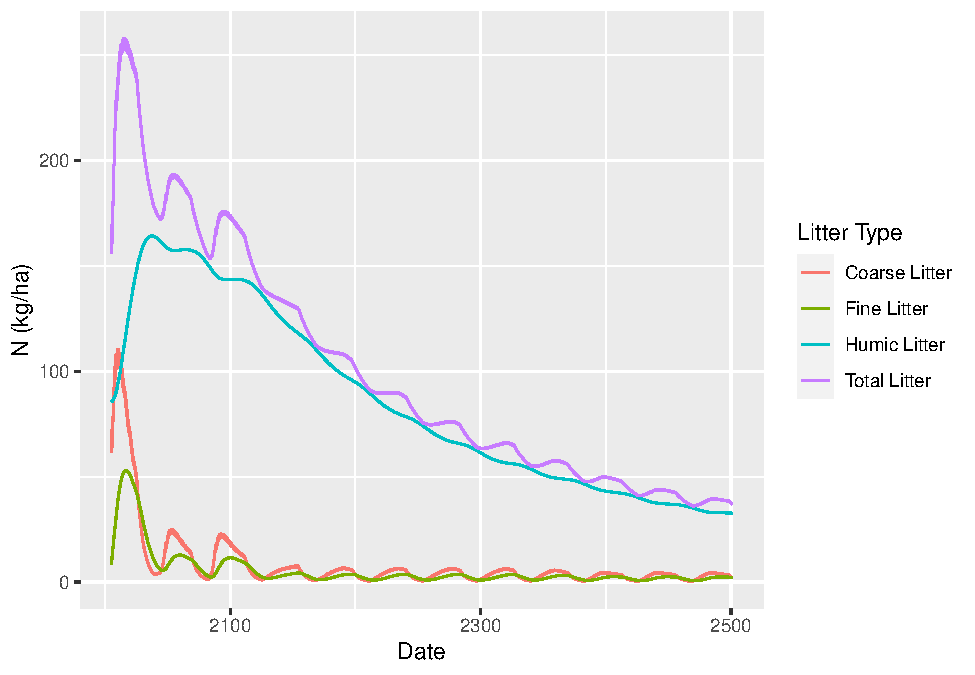
\includegraphics[width=0.5\linewidth]{Master_Report_files/figure-latex/unnamed-chunk-36-1} \end{center}

\hypertarget{cation-exchange-capacity}{%
\subsubsection{Cation Exchange
Capacity}\label{cation-exchange-capacity}}

Not yet complete

\hypertarget{anion-exchange-capacity}{%
\subsubsection{Anion Exchange Capacity}\label{anion-exchange-capacity}}

Not yet complete

\hypertarget{chapter-2}{%
\section{Chapter 2}\label{chapter-2}}

\newpage 
\tableofcontents
\listoffigures
\listoftables
\newpage

\hypertarget{soil-solution-results-1}{%
\subsubsection{Soil Solution Results}\label{soil-solution-results-1}}

\begin{table}[!h]

\caption{\label{tab:unnamed-chunk-40}Average Soil Solution Concentrations of Reliable Months (2005-2006)}
\centering
\resizebox{\linewidth}{!}{
\begin{tabular}[t]{lllllllllllllllll}
\toprule
\multicolumn{1}{c}{ } & \multicolumn{16}{c}{\$\textbackslash{}\textbackslash{}mu\$mol/L} \\
\cmidrule(l{3pt}r{3pt}){2-17}
Soil Layer & Ca & Mg & K & Na & NO3 & NH4 & SO4 & Cl & PO4 & DOC & Al & Si & H+ & pH & R & HR\\
\midrule
\cellcolor{gray!6}{Layer 1} & \cellcolor{gray!6}{14.02} & \cellcolor{gray!6}{18.6} & \cellcolor{gray!6}{17.3} & \cellcolor{gray!6}{46.0} & \cellcolor{gray!6}{1.954} & \cellcolor{gray!6}{1.857} & \cellcolor{gray!6}{24.3} & \cellcolor{gray!6}{55.8} & \cellcolor{gray!6}{0.970} & \cellcolor{gray!6}{402} & \cellcolor{gray!6}{0.01551} & \cellcolor{gray!6}{12.2} & \cellcolor{gray!6}{17.63} & \cellcolor{gray!6}{4.75} & \cellcolor{gray!6}{41.7} & \cellcolor{gray!6}{15.7}\\
Layer 2 & 16.64 & 22.8 & 19.3 & 54.9 & 1.431 & 1.078 & 25.3 & 64.2 & 0.847 & 639 & 0.02971 & 29.5 & 24.91 & 4.60 & 63.0 & 28.3\\
\cellcolor{gray!6}{Layer 3} & \cellcolor{gray!6}{23.27} & \cellcolor{gray!6}{27.4} & \cellcolor{gray!6}{22.4} & \cellcolor{gray!6}{49.8} & \cellcolor{gray!6}{0.980} & \cellcolor{gray!6}{0.719} & \cellcolor{gray!6}{25.3} & \cellcolor{gray!6}{71.1} & \cellcolor{gray!6}{0.658} & \cellcolor{gray!6}{698} & \cellcolor{gray!6}{0.01889} & \cellcolor{gray!6}{42.1} & \cellcolor{gray!6}{19.46} & \cellcolor{gray!6}{4.71} & \cellcolor{gray!6}{71.2} & \cellcolor{gray!6}{28.5}\\
Layer 4 & 9.65 & 16.7 & 15.0 & 48.5 & 0.581 & 0.746 & 12.9 & 71.2 & 0.369 & 425 & 0.02798 & 51.1 & 22.63 & 4.65 & 42.1 & 18.7\\
\cellcolor{gray!6}{Layer 5} & \cellcolor{gray!6}{13.44} & \cellcolor{gray!6}{22.2} & \cellcolor{gray!6}{15.2} & \cellcolor{gray!6}{51.6} & \cellcolor{gray!6}{0.505} & \cellcolor{gray!6}{1.278} & \cellcolor{gray!6}{12.7} & \cellcolor{gray!6}{76.1} & \cellcolor{gray!6}{0.178} & \cellcolor{gray!6}{424} & \cellcolor{gray!6}{0.00642} & \cellcolor{gray!6}{53.1} & \cellcolor{gray!6}{9.34} & \cellcolor{gray!6}{5.03} & \cellcolor{gray!6}{46.7} & \cellcolor{gray!6}{13.9}\\
\addlinespace
Layer 6 & 12.56 & 20.0 & 17.3 & 54.2 & 0.494 & 1.510 & 12.7 & 81.7 & 0.210 & 386 & 0.00813 & 56.7 & 11.12 & 4.95 & 41.9 & 13.3\\
\cellcolor{gray!6}{Layer 7} & \cellcolor{gray!6}{15.97} & \cellcolor{gray!6}{21.8} & \cellcolor{gray!6}{16.2} & \cellcolor{gray!6}{61.0} & \cellcolor{gray!6}{0.491} & \cellcolor{gray!6}{1.947} & \cellcolor{gray!6}{12.7} & \cellcolor{gray!6}{88.0} & \cellcolor{gray!6}{0.243} & \cellcolor{gray!6}{430} & \cellcolor{gray!6}{0.00499} & \cellcolor{gray!6}{61.1} & \cellcolor{gray!6}{7.62} & \cellcolor{gray!6}{5.12} & \cellcolor{gray!6}{48.4} & \cellcolor{gray!6}{13.0}\\
Layer 8 & 15.75 & 20.2 & 18.5 & 68.6 & 0.500 & 2.299 & 12.7 & 92.6 & 0.207 & 426 & 0.00390 & 63.4 & 6.24 & 5.20 & 49.0 & 11.9\\
\bottomrule
\end{tabular}}
\end{table}

\begin{figure}[H]
\includegraphics[width=0.5\linewidth]{Master_Report_files/figure-latex/unnamed-chunk-41-1} \includegraphics[width=0.5\linewidth]{Master_Report_files/figure-latex/unnamed-chunk-41-2} \caption{Figure 1: Monthly Calcium Concentrations by Soil Layer}\label{fig:unnamed-chunk-41}
\end{figure}
\begin{figure}[H]
\includegraphics[width=0.5\linewidth]{Master_Report_files/figure-latex/unnamed-chunk-42-1} \includegraphics[width=0.5\linewidth]{Master_Report_files/figure-latex/unnamed-chunk-42-2} \caption{Figure 2: Monthly Magnesium Concentrations by Soil Layer}\label{fig:unnamed-chunk-42}
\end{figure}
\begin{figure}[H]
\includegraphics[width=0.5\linewidth]{Master_Report_files/figure-latex/unnamed-chunk-43-1} \includegraphics[width=0.5\linewidth]{Master_Report_files/figure-latex/unnamed-chunk-43-2} \caption{Figure 3: Monthly Potassium Concentrations by Soil Layer}\label{fig:unnamed-chunk-43}
\end{figure}
\begin{figure}[H]
\includegraphics[width=0.5\linewidth]{Master_Report_files/figure-latex/unnamed-chunk-44-1} \includegraphics[width=0.5\linewidth]{Master_Report_files/figure-latex/unnamed-chunk-44-2} \caption{Figure 4: Monthly Sodium Concentrations by Soil Layer}\label{fig:unnamed-chunk-44}
\end{figure}

\begin{figure}[H]
\includegraphics[width=0.5\linewidth]{Master_Report_files/figure-latex/unnamed-chunk-45-1} \includegraphics[width=0.5\linewidth]{Master_Report_files/figure-latex/unnamed-chunk-45-2} \caption{Figure 5: Monthly Aluminum Concentrations by Soil Layer}\label{fig:unnamed-chunk-45}
\end{figure}

\begin{figure}[H]
\includegraphics[width=0.5\linewidth]{Master_Report_files/figure-latex/unnamed-chunk-46-1} \includegraphics[width=0.5\linewidth]{Master_Report_files/figure-latex/unnamed-chunk-46-2} \caption{Figure 6: Monthly SiO2 Concentrations by Soil Layer}\label{fig:unnamed-chunk-46}
\end{figure}

\textbackslash begin\{figure\}{[}H{]}
\includegraphics[width=0.5\linewidth]{Master_Report_files/figure-latex/unnamed-chunk-47-1}
\includegraphics[width=0.5\linewidth]{Master_Report_files/figure-latex/unnamed-chunk-47-2}
\textbackslash caption\{Figure 7: Monthly Organic Acid 80\_WTH (R-)
Concentrations by Soil Layer\}\label{fig:unnamed-chunk-47}
\textbackslash end\{figure\}

\begin{figure}[H]
\includegraphics[width=0.5\linewidth]{Master_Report_files/figure-latex/unnamed-chunk-48-1} \includegraphics[width=0.5\linewidth]{Master_Report_files/figure-latex/unnamed-chunk-48-2} \caption{Figure 8: Monthly pH by Soil Layer}\label{fig:unnamed-chunk-48}
\end{figure}

\hypertarget{weathering-results-1}{%
\subsubsection{Weathering Results}\label{weathering-results-1}}

\hypertarget{figures-1}{%
\paragraph{Figures}\label{figures-1}}

\begin{figure}[H]
\includegraphics[width=0.5\linewidth]{Master_Report_files/figure-latex/unnamed-chunk-50-1} \includegraphics[width=0.5\linewidth]{Master_Report_files/figure-latex/unnamed-chunk-50-2} \caption{Figure 9: Calcium Weathering by Layer}\label{fig:unnamed-chunk-50}
\end{figure}

\begin{figure}[H]
\includegraphics[width=0.5\linewidth]{Master_Report_files/figure-latex/unnamed-chunk-51-1} \includegraphics[width=0.5\linewidth]{Master_Report_files/figure-latex/unnamed-chunk-51-2} \caption{Figure 10: Magnesium Weathering by Layer}\label{fig:unnamed-chunk-51}
\end{figure}

\begin{figure}[H]
\includegraphics[width=0.5\linewidth]{Master_Report_files/figure-latex/unnamed-chunk-53-1} \includegraphics[width=0.5\linewidth]{Master_Report_files/figure-latex/unnamed-chunk-53-2} \caption{Figure 12: Aluminum Weathering by Layer}\label{fig:unnamed-chunk-53}
\end{figure}

\begin{figure}[H]
\includegraphics[width=0.5\linewidth]{Master_Report_files/figure-latex/unnamed-chunk-54-1} \includegraphics[width=0.5\linewidth]{Master_Report_files/figure-latex/unnamed-chunk-54-2} \caption{Figure 13: Phosphate Weathering by Layer}\label{fig:unnamed-chunk-54}
\end{figure}

\begin{figure}[H]
\includegraphics[width=0.5\linewidth]{Master_Report_files/figure-latex/unnamed-chunk-55-1} \includegraphics[width=0.5\linewidth]{Master_Report_files/figure-latex/unnamed-chunk-55-2} \caption{Figure 14: Silica Weathering by Layer}\label{fig:unnamed-chunk-55}
\end{figure}

\begin{figure}[H]
\includegraphics[width=0.5\linewidth]{Master_Report_files/figure-latex/unnamed-chunk-56-1} \includegraphics[width=0.5\linewidth]{Master_Report_files/figure-latex/unnamed-chunk-56-2} \caption{Figure 15: Sodium Weathering by Layer}\label{fig:unnamed-chunk-56}
\end{figure}

\hypertarget{litter-pool-results-1}{%
\subsubsection{Litter Pool Results}\label{litter-pool-results-1}}

\begin{figure}[H]
\includegraphics[width=0.5\linewidth]{Master_Report_files/figure-latex/unnamed-chunk-58-1} \caption{Figure 17: Litter Pool Carbon Content Over Simulation Period}\label{fig:unnamed-chunk-58}
\end{figure}

\begin{figure}[H]
\includegraphics[width=0.5\linewidth]{Master_Report_files/figure-latex/unnamed-chunk-59-1} \caption{Figure 18: Litter Pool Ca Content Over Simulation Period}\label{fig:unnamed-chunk-59}
\end{figure}

\begin{figure}[H]
\includegraphics[width=0.5\linewidth]{Master_Report_files/figure-latex/unnamed-chunk-60-1} \caption{Figure 19: Litter Pool Mg Content Over Simulation Period}\label{fig:unnamed-chunk-60}
\end{figure}

\begin{figure}[H]
\includegraphics[width=0.5\linewidth]{Master_Report_files/figure-latex/unnamed-chunk-61-1} \caption{Figure 20: Litter Pool K Content Over Simulation Period}\label{fig:unnamed-chunk-61}
\end{figure}

\begin{figure}[H]
\includegraphics[width=0.5\linewidth]{Master_Report_files/figure-latex/unnamed-chunk-62-1} \caption{Figure 21: Litter Pool P Content Over Simulation Period}\label{fig:unnamed-chunk-62}
\end{figure}

\begin{figure}[H]
\includegraphics[width=0.5\linewidth]{Master_Report_files/figure-latex/unnamed-chunk-63-1} \caption{Figure 22: Litter Pool S Content Over Simulation Period}\label{fig:unnamed-chunk-63}
\end{figure}

\hypertarget{tree-nutrient-content-1}{%
\subsubsection{Tree Nutrient Content}\label{tree-nutrient-content-1}}

\textbackslash begin\{figure\}{[}H{]}

\{\centering \subfloat[Calcium content in each biomass compartment\label{fig:unnamed-chunk-64-1}]{\includegraphics[width=0.5\linewidth]{Master_Report_files/figure-latex/unnamed-chunk-64-1} }\subfloat[Magnesium content in each biomass compartment\label{fig:unnamed-chunk-64-2}]{\includegraphics[width=0.5\linewidth]{Master_Report_files/figure-latex/unnamed-chunk-64-2} }\newline\subfloat[Potassium content in each biomass compartment\label{fig:unnamed-chunk-64-3}]{\includegraphics[width=0.5\linewidth]{Master_Report_files/figure-latex/unnamed-chunk-64-3} }

\}

\textbackslash caption\{80\_WTH Cation Nutrient Content in Simulated
Forest\}\label{fig:unnamed-chunk-64} \textbackslash end\{figure\}

\begin{figure}[H]

{\centering \subfloat[Nitrogen content in each biomass compartment\label{fig:unnamed-chunk-65-1}]{\includegraphics[width=0.5\linewidth]{Master_Report_files/figure-latex/unnamed-chunk-65-1} }\subfloat[Sulfur content in each biomass compartment\label{fig:unnamed-chunk-65-2}]{\includegraphics[width=0.5\linewidth]{Master_Report_files/figure-latex/unnamed-chunk-65-2} }\newline\subfloat[Phosphorous content in each biomass compartment\label{fig:unnamed-chunk-65-3}]{\includegraphics[width=0.5\linewidth]{Master_Report_files/figure-latex/unnamed-chunk-65-3} }\subfloat[Biomass of each compartment\label{fig:unnamed-chunk-65-4}]{\includegraphics[width=0.5\linewidth]{Master_Report_files/figure-latex/unnamed-chunk-65-4} }

}

\caption{N, S, and P Nutrient Contents and biomass per compartment}\label{fig:unnamed-chunk-65}
\end{figure}

\#\#\# Comparison of Inputs and Outputs

\textbackslash begin\{figure\}{[}H{]}

\{\centering \subfloat[Ca Leaching Losses\label{fig:unnamed-chunk-67-1}]{\includegraphics[width=0.5\linewidth]{Master_Report_files/figure-latex/unnamed-chunk-67-1} }\subfloat[Mg Leaching Losses\label{fig:unnamed-chunk-67-2}]{\includegraphics[width=0.5\linewidth]{Master_Report_files/figure-latex/unnamed-chunk-67-2} }

\}

\textbackslash caption\{Annual Leaching Losses of Divalent 80\_WTH
Cations\}\label{fig:unnamed-chunk-67} \textbackslash end\{figure\}

\textbackslash begin\{figure\}{[}H{]}

\{\centering \subfloat[K Leaching Losses\label{fig:unnamed-chunk-68-1}]{\includegraphics[width=0.5\linewidth]{Master_Report_files/figure-latex/unnamed-chunk-68-1} }\subfloat[Na Leaching Losses\label{fig:unnamed-chunk-68-2}]{\includegraphics[width=0.5\linewidth]{Master_Report_files/figure-latex/unnamed-chunk-68-2} }

\}

\textbackslash caption\{Annual Leaching Losses of Monovalent 80\_WTH
Cations\}\label{fig:unnamed-chunk-68} \textbackslash end\{figure\}

\begin{figure}[H]

{\centering \subfloat[N Leaching Losses\label{fig:unnamed-chunk-69-1}]{\includegraphics[width=0.5\linewidth]{Master_Report_files/figure-latex/unnamed-chunk-69-1} }\subfloat[S Leaching Losses\label{fig:unnamed-chunk-69-2}]{\includegraphics[width=0.5\linewidth]{Master_Report_files/figure-latex/unnamed-chunk-69-2} }\newline\subfloat[P Leaching Losses\label{fig:unnamed-chunk-69-3}]{\includegraphics[width=0.5\linewidth]{Master_Report_files/figure-latex/unnamed-chunk-69-3} }

}

\caption{Annual Leaching Losses of N, P, and S}\label{fig:unnamed-chunk-69}
\end{figure}

Not yet complete

\hypertarget{analysis-1-1}{%
\subsubsection{Analysis 1}\label{analysis-1-1}}

\begin{center}\includegraphics[width=0.5\linewidth]{Master_Report_files/figure-latex/unnamed-chunk-71-1} \end{center}

\hypertarget{cation-exchange-capacity-1}{%
\subsubsection{Cation Exchange
Capacity}\label{cation-exchange-capacity-1}}

Not yet complete

\hypertarget{anion-exchange-capacity-1}{%
\subsubsection{Anion Exchange
Capacity}\label{anion-exchange-capacity-1}}

Not yet complete

\end{document}
